\documentclass[oneside,
  digital, %% This option enables the default options for the
           %% digital version of a document. Replace with `printed`
           %% to enable the default options for the printed version
           %% of a document.
  table,   %% Causes the coloring of tables. Replace with `notable`
           %% to restore plain tables.
  nolof,     %% Prints the List of Figures. Replace with `nolof` to
           %% hide the List of Figures.
  nolot,     %% Prints the List of Tables. Replace with `nolot` to
           %% hide the List of Tables.
  %% More options are listed in the user guide at
  %% <http://mirrors.ctan.org/macros/latex/contrib/fithesis/guide/mu/fi.pdf>.
]{fithesis3}
%% The following section sets up the locales used in the thesis.
\usepackage[resetfonts]{cmap} %% We need to load the T2A font encoding
\usepackage[T1,T2A]{fontenc}  %% to use the Cyrillic fonts with Russian texts.
\usepackage[
  main=english, %% By using `czech` or `slovak` as the main locale
                %% instead of `english`, you can typeset the thesis
                %% in either Czech or Slovak, respectively.
  german, russian, czech, slovak %% The additional keys allow
]{babel}        %% foreign texts to be typeset as follows:
%%
%%   \begin{otherlanguage}{german}  ... \end{otherlanguage}
%%   \begin{otherlanguage}{russian} ... \end{otherlanguage}
%%   \begin{otherlanguage}{czech}   ... \end{otherlanguage}
%%   \begin{otherlanguage}{slovak}  ... \end{otherlanguage}
%%
%% For non-Latin scripts, it may be necessary to load additional
%% fonts:
\usepackage{paratype}
\def\textrussian#1{{\usefont{T2A}{PTSerif-TLF}{m}{rm}#1}}
%%
%% The following section sets up the metadata of the thesis.
\thesissetup{
    university    = mu,
    faculty       = fi,
    type          = mgr,
    author        = Martin Štefanko,
    gender        = m,
    advisor       = {Bruno Rossi, PhD},
    title         = {Use of Transactions within a Reactive Microservices Environment},
    TeXtitle      = {Use of Transactions within a Reactive Microservices Environment},
    keywords      = {transactions, Narayana, JTA, reactive, microservices, asynchronous, saga, compensating transactions},
    TeXkeywords   = {transactions, Narayana, JTA, reactive, microservices, asynchronous, saga, compensating transactions},
}
\thesislong{abstract}{
abstract
}
\thesislong{thanks}{
   thanks
}
%% The following section sets up the bibliography.
\usepackage{booktabs}

\usepackage{makeidx}      %% The `makeidx` package contains
\makeindex                %% helper commands for index typesetting.
%% These additional packages are used within the document:
\usepackage{paralist}
\usepackage{amsmath}
\usepackage{amsthm}
\usepackage{amsfonts}
\usepackage{url}
\usepackage{menukeys}
\usepackage{minted}
\usepackage{needspace}

\newcommand{\newlinepar}[1]{\paragraph{#1}\needspace{4\baselineskip}\mbox{}\\}


\begin{document}
\chapter{Introduction}

\clearpage
\chapter{Transaction concepts}

This chapter introduces the basic notions of transactions, their properties and common problems with their management across multiple nodes in distributed systems. 

\section{Transaction}

A transaction is an unit of processing that provides all-or-nothing property to the work that is conducted within its scope, also ensuring that shared resources are protected from multiple users \cite{java_tran_processing}. It represents an unified and inseparable sequence of operations that are either all provided or none of them take effect. 

The transaction can end in two forms: it can be either \textit{commited} or \textit{aborted}. The commit determines a successful outcome - all operations within the transaction have been executed. The abort means that all performed operations have been undone and the system is in the same state as if the transaction have not been started.

Generally, the achievement of the above mentioned features may differ depending on the scope and utilization of the transaction concepts in the application.

\section{ACID properties}

A transaction can be viewed as a group of business logic statements with certain shared properties \cite{nar_wf}. Generally considered properties are one or more of atomicity, consistency, isolation and durability. These four properties are often referenced as ACID properties \cite{haerder_reuter_1983} and they describe the major points important for the transaction concepts.\footnote{Although, the ACID acronym has been associated with transactions since their beginning, Eric Brewer, the inventor of the CAP theorem, discussed in the later section, stated in his article from 2012 that it is "more mnemonic than precise".\cite{cap_12years}}

\subsection{Atomicity}

The transaction consists of a sequence of operations performed on different resources. An atomicity property means that all operations in the transaction are performed as if they were a single unit. 

As the word atomicity is an overloaded term in many computational science branches, some authors prefer to reference it in the ACID context as the abortability property. The abortability is defined as  the ability to abort a transaction on error and have all writes from that transaction discarded \cite{design_data_intens_apps}. This implies that when the transaction commits successfully, all of its operations are also required to execute a valid commit. Conversely, when the transaction fails and needs to be aborted, all realized operations and effects must be undone.

Particularly in the distributed environment, the atomicity property is commonly achieved by the usage of consensus multi-phase protocols. The standardized protocol is the two phase commit protocol (2PC) which is used by the majority of modern transaction systems. The consensus protocols are discussed in detail in the section \ref{sec:consensus-protocols}.

\subsection{Consistency}

The word consistency refers to restrictions placed on data changes that may happen only in allowed ways. When the data is persisted, it must be valid according to all defined rules which meet the application invariants. The consistency property describes that the transaction maintains the consistency of the system and resources that it is being performed on. When the transaction is started on the consistent system, this system must remain consistent when the transaction ends - it moves from one consistent state to another.

Unlike other transactional properties (A, I, D), consistency cannot be realized by the transaction system as it does not hold any semantic knowledge about the resources it manipulates \cite{java_tran_processing}. Therefore, the achievement of this property is the responsibility of the application code.

\subsection{Isolation}

The isolation property takes effect when multiple transactions can be executed concurrently on the same resources. It provides a guarantee that concurrent transactions can not interfere one with another. Therefore each concurrent execution on the shared resource must be equivalent to some serial ordering of contained transactions. This is why the isolation is often also referred to as a serializability.

From the perspective of an external user the isolation property means that the transaction appears as it was executed entirely alone. This means that even if there are multiple transactions in the system executed concurrently, this fact is hidden from the every external view.

As an instinctive extension of the consistency property, the serial execution of the transaction keeps the consistent state. The execution of the transactions in parallel therefore cannot result into inconsistent system.

\newlinepar{Isolation levels}

The ANSI SQL-92 \cite{sql-92} standard distinguishes several levels that describe to which extent the isolation guarantees are provided. Levels are differentiated by simplifications of the locking mechanism in exchange for the faster processing. These levels, in decreasing order, are serializable, repeatable read, snapshot isolation, read committed and read uncommitted isolation. The standard defines distinction between levels by the type of anomalies their are able to prevent. 

In practice, this approach is not always considered as sufficient due to its locking expectations \cite{ansi-sql-critique}. The alternative technique which is not based on locking mechanisms is called the Multi version concurrency control (MVCC). This section describes isolation levels based on the SQL-92 standard but the MVCC will be referenced where applicable.

\newlinepar{Read uncommitted}

This is the lowest level in which the transaction sets the lock only when it needs to modify the data item and releases it immediately after the modification is complete. This allows that one transaction may read the not yet committed changes of any other transaction which is phenomena referred to as the dirty read.

However, the read uncommitted isolation level already prevents the dirty write conflict which represents the transaction the overwrite of the value previously written by another transaction that did not commit. This problem can be easily described on an example depicted in the figure 2.1. In this execution, the resulting data state contains different values for variables (x = B and y = A). However, in any serial execution of transaction the result would be consistent. The read uncommitted level prevents this phenomena as it prohibits access to data items before the former write locks are released.

\begin{figure}
    \begin{center}
        \includegraphics[height=55mm]{images/dirtyWrite.png}
    \end{center}
    \caption{Dirty writes}
\end{figure}


\newlinepar{Read committed}

Read committed level differs from the previous level in that it prohibits dirty reads. It allows to read the data item only when it has been committed. This directly implies that dirty reads are impossible to occur in this isolation level by the definition.


\newlinepar{Repeatable read}

This isolation level prevents the anomaly called the non-repeatable read which may still appear in read committed. The non-repeatable read is a problem of reading the data values in different points of time in which the whole consistent data state may not be ensured. This means that the transaction may read the data change in later point in time which may invalidate already read information from a previous processing.

For example, imagine a bank system with two accounts -- both with starting balance 500 and a transfer of 100 from account 1 to 2 as a transaction. If another transaction reads the balance of the account 2 prior to start of transaction, it will get 500. However, the subsequent read from the account 1 after the transaction has committed would output 400 which would result into inconsistent information.

The MVCC alternative to the repeatable read is the snapshot isolation. Both the repeatable read and the snapshot isolation prevent non-repeatable reads, but they differ in implementation \cite{isolation_levels}. Repeatable read is based on the locking mechanisms which may be complex to maintain. However, the snapshot isolation allows each transaction to read data from a snapshot of the (committed) data which is created at the time the transaction is started \cite{ansi-sql-critique}. The database is required to internally keep track of several states and provide each transaction with the snapshot that is appropriate for its time span.

\newlinepar{Serializable}

On top of the repeatable read, the serializable isolation prevents the system from one more race condition known as the write skew. The basic principle of a write skew is a transaction that reads data from the storage and then makes a decision based on this information. However, different transactions may write the result into different parts of the database which means they can not conflict. The problem is that by the time the transaction commits, the premise of the decision may no longer be true and the resulting state may break the integrity constraints of the database.

\subsection{Durability}

This property characterizes that all changes done by the transactions must be persistent, i. e. any state changes performed during the transaction must be preserved in case of any subsequent system failure. How the state is preserved usually depends on the particular implementation of the transaction system. Generally, to achieve this property the use of the persistent storage like a disk drive or a cloud is sufficient. Even if this kind of storage is acceptable, it still can not prevent data loss in the case of more critical catastrophic failures.


\section{Transaction manager}
\label{sec:transaction-manager}

A transaction manager (TM) is a component responsible for the transaction processing, coordination and their sequential or parallel execution across one or more resources. It ensures the proper and valid completion of each transaction. It is also liable for making the final decision whether to commit or rollback the transaction. Clients often communicate with the transaction manager only when they need to start or end the transaction.

Main responsibilities of the transaction manager are starting and ending (commit or abort) of transactions, the supervision of transactions scoped across multiple resources and rollback capabilities ensuring the failure recovery. 

%It also manages the transaction context which represents the identification and contains the state of the transaction.

\subsection{TM types}

A local transaction manager or a resource manager is responsible for the coordination of transactions concerning only a single resource. Because of the range of its scope, it is often built in directly into the resource. The span of the resource is defined by the managing platform, e. g. the JMS context or the JDBC database connection.  

The restriction of the local TM scope does not intend its application across multiple resources. This means that it cannot provide ACID guarantees if the transaction contains, for instance, both the database update and the JMS message send as these resources are handled by different resource managers.

The management of transactions over multiple resources is supported by a global transaction manager. It represents an operation external component that is able to coordinate several resource managers in order to provide ACID transactions spanning two or more different transactional resources.

\subsection{JTA and JTS}

The definition and management of transactions with a guarantee of all ACID properties is in the Java environment represented by two Java EE specifications: the Java Transaction API (JTA) and the Java Transaction Service (JTS). 

The JTA is a specification which defines high-level interfaces between a transaction manager and the parties involved in a distributed transaction system: the application, the resource manager and the application server \cite{jta}. It also determines the Java mapping of the industry standard X/Open XA protocol which allows local resource managers to participate in the global transaction managed by an external transaction manager.

The JTS represents a specification of the transaction manager implementation which supports the JTA specification at the high-level and implements the Java mapping of the Object Management group (OMG) Object Transaction Service (OTS) specification at the low-level \cite{jts}. It uses the Common Object Request Broker Architecture Object Transaction Service (CORBA OTS) interfaces for the interoperability and portability of the transaction context between different JTS transaction managers over the Internet InterORB Protocol (IIOP).

\subsection{XA specification}

The eXtended Architecture (XA) standard is the X/Open Common Applications Environment (CAE) specification published in 1991 which describes the bidirectional interface between a transaction manager and a resource manager \cite{xa_spec}. It maintains two types of components that clients can interact with: the transaction manager (TM) which defines the global TM in a sense described in the previous section and the XA resources that represent local resource managers.

The resource manager implements the XA interface in order to provide a switch that effectively delagates the transaction control to the TM. The XA TM coordination is based on the two phase commit protocol (2PC) which means that the XA interface contains all necessary function calls that needs to available for 2PC -- \texttt{xa\_prepare}, \texttt{xa\_commit} and \texttt{xa\_rollback}. The Java mapping of the XA standard is present in the class \texttt{javax.transaction.xa.XAResource}.



\section{Transaction models}

From the development point of view, there exist three distinct transaction models that may be used in the Java environment. The transaction model defines rules and semantics of how developers declare and work with transactions. These models are local, programmatic and declarative transactions. This chapter describes each model respectively and examines how it can be applied in Java applications.

\subsection{Local transaction model}

The local transaction model derives its name from the fact that transactions are managed by a local resource manager described in the previous section. This approach represents the transaction as a connection to the individual resource. Common use-cases for this model include the Java database connectivity (JDBC) or the Java Message Service (JMS) connection providers.

The connection is usually by default configured to commit or rollback the local transaction after each operation, e. g. a database query or sending a message to a queue. The interaction with the local manager may differ depending on the underlying resource. For instance, the JMS \texttt{Session} interface provides both methods \texttt{commit()} and \texttt{rollback()} that process or destroy included message operations respectively.

The major drawback of this model is that local transactions cannot be joined into the single ACID transaction that spans over multiple resources using the XA global transaction \cite{java_transaction_design_strategies} (e. g. we need to update a database and propagate this information to the JMS topic). Another important problem is the requirement of the manual transaction management in the application code base.

\subsection{Programmatic transaction model}

The programmatic transaction model (also referenced as the Bean-Managed transaction (BMT)) is introduced by the JTA transaction service implementation. In this model, the developer handles the complete management of the transaction in the source code.

Although the JTA specification provides a range of APIs, the only required interface for the utilization of the programmatic transactions is the \texttt{javax.transaction.UserTransaction} \cite{jta}. This interface represents an abstraction for the developer to programatically control transaction boundaries. The only concerned methods are \texttt{begin()}, \texttt{commit()}, \texttt{rollback()} and \texttt{getStatus()}. The call to the \texttt{begin()} will start a new transaction and associates it with the current thread. As the Java platform allows only one transaction to be associated with the thread, a call to the \texttt{begin()} method may result into exception in case the transaction has already been started in the current context. The transaction end methods (\texttt{commit()} and \texttt{rollback()}) perform their respective actions and disassociate the transaction with the thread. The \texttt{getStatus()} method returns an integer value representing the status of the current transaction derived from  \texttt{javax.transaction.Status} class \cite{jta}.

The most important problem introduced by the programmatic model is that the developer must ensure that the transaction is always terminated in the method that started the transaction \cite{java_transaction_design_strategies}. This is often the case when  the initiating method ends up with an uncaught exception and for this reason, the transaction needs to be committed or rollbacked before the method returns.

\subsection{Declarative transaction model}
\label{sec:decl-tran-model}

The declarative transaction model is also referred to as the Container-Managed Transactions (CMT). In this model, the supplying, underlying container manages all transactions on the users behalf. This includes starting and the administration of the end phases (either commit or rollback) of transactions. The developer is only required to setup the container with the transaction configuration that declares, for instance, that the transaction should be rollbacked on any exception.

The main interface that is utilized in declarative transactions is the \texttt{javax.transaction.TransactionManager}. Although this interface provides  same methods that are present in the \texttt{UserTransaction} interface used in the programmatic model, users are strongly encouraged to use it only in CMT. In addition to the \texttt{UserTransaction}, it introduces two methods that manage the transaction suspensions. The \texttt{suspend()} method suspends and  disassociates the transaction with the current thread. It returns an object that represents the identification of the running transaction. This transaction object can be afterwards used as an argument to the \texttt{resume()} method to associate the transaction again with the current thread and continue the transaction execution. In practice, CMT transactions are generally defined by specific annotations and the direct use of \texttt{TransactionManager} interface is discouraged.

Another essential method that is often associated with the container transactions is the \texttt{setRollbackOnly()}. It declares that the only possible transaction result is to rollback and any consequent actions can not change it.

With the declarative transaction model, the users are required to configure the container with the settings of how individual transactions should be managed. This can be set up through the transaction attribute represented by, for instance, \texttt{TransactionAttributeType} (Enterprise Java Beans (EJB)), \texttt{Transactional.TxType} (Context and Dependency Injection (CDI)) or \texttt{TransactionDefinition} (Spring) classes. The supported values are -- Required, Mandatory, RequiresNew, Supports, NotSupported and Never\footnote{Spring adds one more transaction attribute called Nested which represents a single physical transaction with multiple savepoints that it can roll back to \cite{spring_transaction_management_documentation}}:

\begin{itemize}
    \item \textbf{Required} -- If the transaction context is already present on the invocation, it will be used. Otherwise a new transaction is started. This is the most characteristic attribute and it usually configured as a default value.
    
    \item \textbf{Mandatory} -- Similarly to the Required, mandatory transaction attribute represents that the transaction must be present on the execution. However, it requires that the transaction is already started prior to the invocation. Alternatively, it throws \texttt{TransactionRequiredException} if the transaction context can not be found.
    
    \item \textbf{RequiresNew} -- The container will begin a new transaction on every invocation. If there is already a transaction context present, it is suspended for the duration of the processing of the new transaction. This breaks the atomicity property of the former transaction.
    
    \item \textbf{Supports} -- This attribute represents an invocation that is not required to run under the transaction context. It tells the container to use the transaction context, if it exists before the call, or to execute the operation non-transactionally if the transaction is not present.
    
    \item \textbf{NotSupported} -- The method will not be executed within the transaction context. If the transaction exists prior to the invocation, it is suspended and the method is invoked. In other case, the method is immediately started without the initiation of a new transaction.
    
    \item \textbf{Never} -- The container is forbidden to invoke the method if there is a transaction context present. In contrast with the NotSupported attribute which only suspends former transaction, this attribute will throw a runtime exception when the transaction is present before the invocation.
\end{itemize}

\section{Distributed transactions}

Transaction concepts, presented in the previous sections, can be certainly expanded to the distributed environment. The distributed transaction represents an ACID transaction that is executed over a number of independent participants connected through a communication network. The main disadvantage of these transactions is their liability to frequent failures of individual nodes or communication channels that connect them -- which is something that the distributed transaction processing (DTP) needs to account for. 

Each node is associated with a transaction manager (TM) that manages a local transaction and communicates with other TMs in order to perform a global transaction. Generally, there is one TM selected as a global coordinator that administers TMs participating in the distributed transaction. The coordinator can be allocated with the participating node or can act as a standalone service.

The accomplishment of ACID properties with the frequent partitions failures is very difficult to achieve. In order to achieve the atomic outcome, all of the participating nodes needs to achieve a shared consensus on whether it is possible to execute a successful commit. Even if the DTP system is able to provide the distributed consensus, it often comes with a performance cost. This lead to the commonly hesitant utilization of the DTP concept in distributed applications in the past. 

However, recent network speeds and computational capacities are increasing. This allows consensus protocols (2PC, Paxos) and other DTP solutions (e.g. sagas) to be easily employed in modern, scalable distributed applications.



\section{Consensus protocols}
\label{sec:consensus-protocols}

The consensus problem represents the procedure of achieving the  agreement for the shared data value between several components. It has its application in many environments including transactions where the TM needs to conclude whether a transaction can be committed depending on the participants consensus.

A consensus protocol describes a series of steps that solve the consensus problem. These steps can be typically divided into three phases -- the selection of candidate values, the exchange of values between participants and the agreement. The final decision of each participant is irreversible. The consensus protocol is correct, if it complies with these conditions \cite{distributed-computing}:

\begin{itemize}
    \item \textbf{Agreement} - all non-faulty\footnote{Some nodes may provide invalid or intentionally wrong information -- these are known as \textit{Byzantine failures} \cite{byzantine-generals-problem}} nodes decide on the same single value
    \item \textbf{Validity} - if all non-faulty nodes have the same initial value, then the consensus must be reached on this value
    \item \textbf{Termination} - all non-faulty nodes eventually decide
\end{itemize}


In the transactions environment, the consensus represents the shared decision whether to commit or rollback the transaction. The following sections describe some of the mostly widely used consensus protocols that may be employed in (potentially distributed) transactional systems.

\subsection{2PC}

The \textit{Two phase commit protocol} is one of the most known employed consensus protocols used not only in the transaction processing. The procedure consists of two phases:

\begin{itemize}
    \item \textbf{The prepare phase} - All participants send their proposals to the coordinator (TM) in which each of them states either that it is able to proceed and commit its work segment or that the transaction needs to be aborted.
    
    \item \textbf{The commit phase} -- After collecting all proposals, the transaction coordinator makes a final decision -- if all participants are able to commit, the transaction can be committed; conversely, if any participant stated that it needs to abort, the transaction is aborted. The final outcome is subsequently forwarded to every participant and the transaction can be finished.
\end{itemize}

The 2PC protocol is able to handle node failures to some extent through the use of transaction log. However, this do not cover every scenario and certain failures may require manual intervention.

The algorithm expects one node to act as a coordinator. This does not necessarily need to be an elected participant. Any node can act as a coordinator and initiate 2PC prepare phase by asking other participants for their votes. Furthermore, there also exits a decentralized variant but with higher massage complexity.

The main disadvantage is that the 2PC is a blocking protocol as it can not proceed when the coordinator is unavailable. If the coordinator fails after the first phase is completed, all participants will block waiting for the coordinator's decision and can not progress (e. g. release locks) until it recovers.

\subsection{3PC}

The \textit{Three phase commit protocol} is a consensus protocol introduced in 1982 by Dale Skeen \cite{3PC}. It extends the 2PC protocol in a non-blocking way -- it allows participants to place upper time bounds on the phases completion which assures that resources are not  held indefinitely. The three phases are:

\begin{itemize}
    \item \textbf{The prepare phase} -- Same as in the 2PC protocol.
    
    \item \textbf{The pre-commit phase} -- If all participants voted in the first phase to commit the transaction, the coordinator sends to every participant a \texttt{preCommit} massage. After the participant receives \texttt{preCommit}, it will proceed by preparing the commit by locking the required resources assuring that it is able to finish the commit. By this stage the participant can not execute any irreversible actions. If the preparation was successful, it responds to the coordinator with the acknowledgment message.
    
    \item \textbf{The commit phase} -- After the coordinator receives preparation confirmation from all participants (the original paper \cite{3PC} allows also to specify a majority vote count), it will commence the commit phase by sending the \texttt{commit} or \texttt{abort} messages, same as in the 2PC protocol.
\end{itemize}

The termination is achieved by the timeout boundaries set on every message expedition. If the coordinator timeouts, it always assumes the rollback outcome -- after the first phase it cannot proceed as it did not receive votes from every participant and after the second phase if the coordinator fails, the state of the protocol would not be recoverable. However, the participant behaves in the same way after phase one (as it did not receive the outcome from the coordinator, it must assume abort) but if it timeouts after the second phase, it proceeds with the commit. This is allowed as the \texttt{preCommit} message is sent by the coordinator only if all participants wanted to commit the transaction in the phase one.

If the coordinator fails, the new coordinator is selected by any election algorithm. This recovery node can determine the outcome of the protocol based on the state of other nodes -- if any node received a \texttt{preCommit} message, the transaction can be committed (all other participants must have also received the \texttt{preCommit} message). If some node did not receive the \texttt{preCommit} message, the transaction can be aborted.

By contrast to the 2PC protocol, the 3PC is resilient to more types of failures. Nevertheless, it cannot withstand the network partition. If the partition disassociate nodes that did receive the \texttt{preCommit} message from those which did not, the newly selected coordinators on each side of the partition will result into opposite outcomes and thereby an inconsistent system. The resilience capabilities are at the expense of the performance cost which approximately two times higher that in the 2PC protocol \cite{3PC}.

In 1998, Keidar and Dolev introduced an \textit{Enhanced three phase commit} protocol (E3PC) which maintains the consistency in the face of site failures and network partitions \cite{E3PC}. It is using two additional counters that impose linear order on the majorities of the system node while still preserving the same computational complexity as 3PC. 


\subsection{Paxos}

The Paxos represents a family of distributed algorithms designed to solve the consensus problem. It has been introduced by Leslie Lamport in 1998 \cite{Paxos}.

The idea of the basic variant of the algorithm is reasonably simple. The Paxos distinguishes three types of system nodes: proposers, acceptors and learners. One node can be of more than one type, even act as all of them. Proposers act as client representatives proposing values that the client wants the system to agree on. Acceptors serves as the voting mechanism and all nodes must know the number of acceptors that form a majority. Learners serve as the representatives that can be queried for the decided value. The algorithm runs in two phases:

\begin{itemize}
    \item \textbf{The promise phase} -- The proposer first sends its proposed value with a new unique identification number generated from a sequence to all acceptors (or the majority). When the acceptor receives a proposed value, it first checks whether the received id number is higher than the last id it promised to ignore. In that case it will respond to the proposer with the \texttt{promise} message which denotes that it will ignore any newly received messages with lower ids. Otherwise, it already promised to the higher proposed id and therefore no action is taken.
    
    \item \textbf{The commit phase} -- If the proposer collects promises from the majority of acceptors, it sends the \texttt{accept-request} message to all acceptors (or the majority) with the same id and the proposed value. When the acceptor receives the \texttt{accept-request} message and it did not already promised to ignore the received id, it sends the \texttt{accept} message to the proposer and all learners. If the id in the message is lower than the promised id, the message is ignored. As the \texttt{accept-request} message is send to the majority of acceptors and all of them accept the value, the consensus is reached.
\end{itemize}

If the acceptor accepts a value, it appends the accepted id and value to each subsequent \texttt{promise} message sent to new proposers. In this case, the proposer knows that there is some value already decided in the system and it continues the processing with the value received in the \texttt{promise} message containing the highest of all received ids. If it wants to update this value, it needs to initiate a new run of the algorithm after the current one has ended. 

Many variants of the Paxos algorithm allows it to sufficiently handle various types of failures that may influence the achievement of the consensus. In particular, even the basic variant handles problems of the 3PC algorithm, namely, network partitions and the restriction to the fail-stop model. Instead, the Paxos protocol is resilient to the fail-recover model which allows individual nodes to recover and continue processing from the point of the failure -- which is expected in the modern distributed systems.

The problem that the algorithm can not solve is two proposers that actively compete for the highest proposal number. This happens between phases as the participants \texttt{accept-request} is rejected due to the higher \texttt{promise} issued to the other proposer. The system is blocked until the conflict can be resolved, e. g., by the exponential back off mechanisms which allows one proposer to wait sufficiently long for the other one to finish. Acceptors are also required to have a persistent storage to avoid providing misleading information in case of the fail-recovery.

\subsection{Conclusions}

This section presented in detail three consensus protocols that can be employed to solve the transaction commit / abort consensus in the distributed systems. There also exists many other algorithms, for instance, the Raft or the Ark which can not be discussed due to the space limitations. The summary of the presented algorithms is available in the table \ref{tab:consensus-protocols-comparison} (this table represents scenarios without any failures).

\begin{table}
    \begin{tabularx}{\textwidth}{lllX}
        \toprule
        Protocol & Time (phases) & Message complexity & Client delay \\
        \midrule
        2PC & 2 & $3(n - 1)$ & 3 RTTs \\
        3PC & 3 & $5(n - 1)$ & 5 RTTs \\
        Paxos & 2 & $4(f + 1)$ ($f$ = majority) & 4 RTTs \\
        \bottomrule
    \end{tabularx}
    \caption{Consensus protocols comparison}
    \label{tab:consensus-protocols-comparison}
\end{table}

The consensus is a very sophisticated and complex problem particularly in distributed environments. As it will be presented in the following chapters, the saga pattern \cite{sagas_publ} provides a simple and elegant alternative to the distributed consensus for the long lived transaction commit.



\clearpage
\chapter{Microservices architecture pattern}

This chapter introduces the concept of microservices and it focuses on why modern, elastic and resilient enterprise systems should be designed and implemented according to this pattern. It provides an updated microservices status overview from my previous work publication \cite{bachelor_thesis}.

\section{Architectural pattern}

Microservices are an architectural pattern which offers an intuitive approach to common problems following a software development. They represent a subset of a Service Oriented Architecture (SOA) \cite{soa} that advocates creating a system from a collection of small, isolated services, each of which owns their data, and is independently isolated, scalable and resilient to failure \cite{reactive_ms_arch}. Instead of the SOA, which builds the applications around the system logical domain, microservices are focused around the application business model. Each microservice represents the separated and independent part of the system that interacts with other components only through predefined communication interfaces\footnote{throughout the rest of this publication we will be using terms \textit{microservice} and \textit{service} interchangeably}.

\subsection{Monolithic architecture}

The effective way of describing why the microservice architecture is emerging as a practical development style, is to begin with the definition of the opposite pattern -- the monolithic architecture. When the application is developed in the monolithic fashion, all of its content is being implemented and deployed as a single archive. Every component, i. e., a unit of software that is independently replaceable and upgradeable \cite{microservices}, is tightly coupled within the application. Because of the easy development of the monolithic software, this approach has been preferred by the majority of edging enterprise applications. However, when the application requires to add a new functionality or to fix a problem, any additional maintenance represents an issue. For instance, even because of the minor change or update in the single component, the scalability, continuous deployment and the general advancement of the whole application can stagnate. 

Monolithic applications present a few advantages -- the development model is often easy to adjust to the application requirements\footnote{the traditional development model represented as the client-server-database or the Model-View-Controller architecture \cite{mvn_architecture}}, the deployment is reduced to single archive (or a small number of archives) and it is easy to horizontally scale by adding more servers behind a shared load balancer. The problems arise when the system becomes large. The monolithic code base is often complex and hard to understand which results into long learning curves \cite{learning_curve} and developer concerns. The automatic deployment and the continuous delivery (CD) of the system also decelerate -- in order to update one component you have to redeploy the entire application \cite{monolithic_arch}. Although, it is still able to scale horizontally, the replicated server instances take up more resources and overload the container with a slower start up speeds. In general, the monolith also represents a commitment to a particular technology (or even its specific version) which makes the system difficult to maintain and also adapt to new emerging technologies.


\subsection{Microservice architecture}

Microservices introduced the application separation into the self-maintained units – services \cite{intro_to_microservices}. The service is a single scalable and deployable unit, which is not dependent on any context. This means that services may be deployed and scaled independently of each other, and may employ different middleware   stacks for their implementation \cite{ms_arch_ecommerce}. 

The important attribute of the microservices system is a service isolation. Each microservice is responsible for the management of its own resources and it is prohibited to directly access resources of any other service. This means that each data request must be processed by the operating microservice which is allowed to accordingly control the data access and computation requirements. Services often correspond to components in the monolithic architecture.

Microservices further extends the Law of Demeter which intents to organize and reduce dependencies between classes \cite{law_of_demeter}. As the service presumably requires to communicate with other services in order to provide system functionality, this law naturally applies to minimize such coupling among microservices on the distributed component level. 

Another standard object-oriented rule that also applies in the microservices environment is the Single Responsibility Principle (SRP) as defined by Robert C. Martin -- a class should have only one reason to change \cite{agile_ppp_c}. There is a common misconception associated with the microservice architecture -- the word \textit{micro} should conform to the service size. Although, this statement is true to some extent (there is no point in creating the microservice of the same size  as the monolith), the \textit{micro} should more resemble a scope of the service responsibility. This concept also corresponds to the Unix philosophy: Make each program do one thing well \cite{unix_time_sharing_foreword}.

The separation and loose coupling of microservices provide an ability to deploy each individual service to the production environment autonomously, not affecting other applications or services. This allows isolated teams to develop, maintain and upgrade services independently and to form these teams around the system problem domains. 

As microservices represent a stateful entities, to achieve data isolation each service exposes an application programming interface (API) through which it is exclusively able to provide functionality to other services. These APIs are often technology-agnostic to ensure that the technology choices are not constrained \cite{building_ms}. Instead of in-process calls employed in the monolithic architecture, applications based on the microservices style utilize services by remote procedure calls which are often asynchronous. This form of segregation also facilitates the system failure recovery or resilience as each particular microservice breakdown is less prone to influence the rest of the system.

\section{Principles of microservices}

This section describes the microservices architecture from the perspective of the business use cases and the solution architecture. It is based on the work of Sam Newman \cite{building_ms, principles_of_microservices} in which he proposed to build each microservices system on a set of principles. This principles may differ for various systems (depending of the application and microservices use cases) but in general, they can reduced to these eight principles:

\begin{enumerate}
	
	\item \textbf{Modeled around the business concepts} -- When the  microservices applications, together with the teams that are responsible for their maintenance, correspond to the business domain, they are generally more stable -- the requirements on their functionality do not change frequently. This allows developers to focus on the particular system segment, rather than on some specific technology stack. Additionally, it also permits services to directly reflect the business requirements.
	
	\item \textbf{Adapting a culture of automation} -- Because of the  service motion, failures or the communication distribution through the network, microservices brings additional complexity to the system. When the number of services increases, the maintenance, administration and deployment can became unmanageable. The automation then presents an essential part of the service life cycle. The practices as the automated service testing, the employment of the continuous delivery or the unification of the deployment strategy over services, allow enterprise systems to scale more efficiently and speed up the mechanism of the service coordination.
	
	\item \textbf{Hiding the internal implementation details} -- Every microservice generally needs to interact with other services or external systems to provide its functionality to the rest of the system. In order to keep the option of independent development, it is essential that each service hides its implementation details. This can be achieved through the motion of bounded contexts as defined for the Domain-Driven design (DDD) \cite{ddd}. The bounded context delimits the applicability of a particular model so that team members have a clear and shared understanding of what has to be consistent and how it relates to other contexts. The context is separated by an explicit interface represented as an API which allows teams to specify which utilities of the service can be shared and which must be hidden. Every request for the service data must be subsequently processed through this public interface.
	
	\item \textbf{Decentralizating all things} -- Microservice architecture is build around the idea of self-sustaining development which means that services are maintained autonomously. This allows to delegate decision making and authority to the team that is accountable for the service maintenance. The team is then able to take full ownership of the service which with the support of the independent deployment mechanism results into the convenient development, testing and life-cycle management. This principle accentuates that relevant business logic should be kept in services themselves and the communication between them must be as simple as possible. This permits to design systems in a way that adheres to the Conway's law  stated in 1967 \cite{conways_law}:
    
    \begin{displayquote}
       Any organization that designs a system (defined broadly) will produce a design whose structure is a copy of the organization's communication structure.
    \end{displayquote}

    This principle also affect the system architecture and design. The purpose is to avoid approaches like enterprise service bus (ESB) or other orchestration systems, which can lead to centralization of business logic \cite{building_ms}. In general, architectures build on the choreography patterns rather than orchestration are preferred. The comparison of these two approaches has been investigated in many research works \cite{chor_and_orch, service_oriented_design, realtime_ws_orch}.
	
	\item \textbf{Independent deployments} -- This is the most important principle of the mircroservices architecture. When the service is being deployed, it should be the requirement that it cannot influence the lifespan of any other service. To achieve this, various techniques like consumer-driven contracts or co-existing endpoints can be used. Consumer-driven contracts make services to state their explicit expectations. These requirements are supported by the provided test suite for individual parts of the domain and they are run with each Continuous integration (CI) build. Co-existing endpoints model accommodates consumers to service changes over time. The idea is to make new endpoint which can process updated client requests while the former endpoint still functions for a limited lifespan. This includes techniques as blue/green releases \cite{blue_green} or canary deployments \cite{canary_deploy}. Customers can utilize both endpoints depending on the version their applications require which allows them to decide when to upgrade. Once the previous endpoint is no longer in use, it can be safely removed.
	
	\item \textbf{Customer first} -- Services exist to be called. It is indispensable to make these calls as simple as possible for the customers. The developers can advatage from any feedback from the clients that use their service. To ease the understanding of the service API, it should be supported by a good documentation provided by API frameworks like Swagger \cite{swagger}. This also includes the service discovery mechanisms to propagate system services and to make the discovery of the service providers more apparent. To combine this information we can use the humane registries \cite{humane_registry} which indicate the human interaction. 
	
	\item \textbf{Failure isolation} -- Even if microservices force distributed isolated development, the architecture still needs to protect against the failure propagation between services. This principle supports resources separation to avoid the single point of failure and it is also supported by the service location distribution. As services require to communicate remotely, it is important to account for the network failures. To prevent cascading failures various techniques like timeouts, bulkheads or circuit breakers \cite{release_it} may be employed. As there are many vulnerabilities in applications which cannot be considered, there is no precise manual on how to attain this principle.
	
	\item \textbf{High observability} -- Monitoring is an important part of development and production deployment. Because of the microservices system distribution, it is not sufficient to observe actions performed by particular services apart. Instead, the monitoring solution must record the system operations altogether. To make this information more accessible, the aggregation is essential. Storing all log entries and statistics in one place can highly impact the monitoring process. Another relevant issue is to track the service calls as the services typically communicate with other services. This can be achieved by mechanisms as semantic monitoring and techniques like synthetic transactions or correlation IDs \cite{building_ms}. By logging this kind of information we can ensure traceability in the case of service failure.
	
\end{enumerate}

\section{Reactive microservices}

Before the definition of what the reactivity means in distributed microservices environments, it is appropriate to start from the basics of what the reactivity signifies in general terms and how these principles may be applied in software architectures. This section introduces the motion behind the reactive design and why it is suitable for the use in the microservices environment.

By the definition in the Oxford dictionary, the word \textit{reactive} symbolizes an exposure of a response to a stimulus or an action in response to a situation rather than creating or controlling it. This definition naturally translates to software systems. However, the interpretation of what the stimuli is in software applications may differ. It might be, for instance, events, messages, requests or failures. The important common property of these impulses is that the development model cannot be implemented in a way to control them. This motions differ from the traditional style of programming models in which the program functioned as a sequence of commands that were always executed in the predefined order and in the maintained, controlled state.

In software systems we distinguish three distinct classes of reactive concerns -- reactive systems, reactive programming and reactive streams \cite{reactive_landscape}. 

\subsection{Reactive systems}

Reactive systems are an architectural style that focuses on the responsiveness. By the definition provided in the Reactive Manifesto \cite{reactive_manifesto}, reactive systems are also resilient, elastic and message driven which makes them more flexible, loosely-coupled and scalable. Generally, this model provides a straightforward programming interactions and simplified dependency management that is required in modern applications. The following enumeration explains these essential properties in detail:

\begin{itemize}
    \item \textbf{Responsiveness} is the most important characteristic of reactive systems. It provides a guarantee of a timely response to normal user requests, as well as the rapid failure detection. Reactive systems are expected to establish a sufficient upper bound placed on the system response times to institute an end user assurance in the system usage.
    
    \item \textbf{Resilience} covers the responsiveness of the system in the case of the system failure. The manifesto states that the system is not resilient, if it becomes unresponsive after any failure. Resilience can be achieved by, e.g., replication, isolation, delegation and loose-coupling. This ensures that the failure in one part of the system cannot effect the system as whole which shadows the component clients from any form of the failure handling.
    
    \item \textbf{Elasticity} involves the system responsiveness in the case of alternating load. Reactive system is expected to be able to dynamically adjust and scale system resources according to the request traffic. Elasticity also implies that the system must be able to actively replicate and regulate its components and distribute user inputs among them by the scalable, predictive (and possibly reactive) algorithms.
    
    \item \textbf{Message driven} elaborates on the asynchronous message exchange between the system components that promotes the loose coupling, isolation and location transparency. Explicit message utilization has many advantages, e.g., flow control, load management or monitoring and engagement of the back pressure. The location transparency, based on virtual addresses, decouples individual components. It may also provide a failure management mechanism, in which case the service cannot distinguish between the communication with a single component or a cluster. Additionally, the asynchronicity allows the system to utilize resources in a non blocking way, only when they are required for the request processing. 
\end{itemize}

\subsection{Reactive programming}

Reactive programming is a development model focusing on the observation of data streams, reacting on changes, and propagating them \cite{building_reactive_ms_in_java}. In the rest of this section, we will be referencing these data streams in the Reactive Extensions methodology as \textit{observables}. An observable is an object that contains dynamically versatile data that represent state which may be of interest to other object. In order to consume the data emitted by an observarble, the interested object must \textit{subscribe} to it.

In practice, reactive programming distinguishes three kinds of observable objects -- observable data streams, singles and completables. Observable, as a stream of data, represents an asynchronous reaction. It provides three handlers, namely, for the data result, error handling and the end of the data stream. The single is a special type of observable that depicts the stream of one value. It is associated with an execution of asynchronous operation which provides data and error callback handlers. The completable observable symbolizes the stream without any value. It contrast with the single, it do not return a data value. For this reason, the completable should be configured with the completion and error handlers.

The observable stream can be of two types -- a cold or hot observable. The cold observables are lazy loaded. This means that the data stream do not process any tasks until somebody starts observing it. It represents an asynchronous action that is invoked only when there is a consumer interested in the result. When an object subscribes to a cold observable, it receives all data objects contained in the stream which allows them to be shared. Conversely, the hot observable data stream is active before the consumer subscriptions. When the consumer subscribes to the hot observable, it will receive all data values from the stream that are emitted after the subscription. Both cold and hot observables require the user subscription to receive the data values from the streams. If the consumer does not subscribe to an observable stream, the data is lost.

The most important concept of reactive programs is the asynchronicity. On the contrary from the traditional program invocations, this processing model is based upon notifications that are emitted when the data stream produces a value. Each asynchronous operation happens independently of the main program flow which introduces several new aspects that needs to considered for this kind of programming paradigm. These aspects can be summarized in three simple rules: avoid side effects\footnote{The side effect is any interaction of the function with the remainder of the program in other way than through its arguments or its return value}, avoid using too many threads and never block.

One of the most popular implementations of the reactive programming principles in modern systems is the Reactive eXtension (RX). It represents a library for asynchronous and event-based programs by using observable sequences \cite{rxJava}. These extensions combine the observer and iterator patterns with a range of functional idioms to allow developers to easily adapt reactive methods. Reactive extensions provide a broad range of implementations for various programming languages as, for instance, Java (RxJava), C\# (Rx.NET) or Kotlin (RxKotlin). 

To conclude, it is important to remember that reactive programming does not build a reactive system \cite{5thingsAboutRP_RHDev}. It only provides a development model that can be used for asynchronous processing, a task based concurrency model or the non-blocking Input/Ouput (I/O) that may be employed with other reactive principles to create responsive and reliable distributed systems as defined in the Reactive Manifesto.

\subsection{Reactive streams}

Reactive streams represent an initiative to provide a standard for asynchronous stream processing with non-blocking back pressure\footnote{Back pressure is a form of feedback mechanism that allows consuming object to regulate the load which is beign sent to it. It is typically employed in situations where the publishing object (observable) is able to emitt data items more quickly than the consuming side is able to process them} \cite{reactive_streams}. It addresses the issue of controlling the load placed on the stream destination in case of the consumption overload. The main focus of reactive streams is placed on the mediating the stream of data among different API components without the requirement to buffer unreasonable amount of data on the receiver side. 

This specification aims to provide a minimal set of interfaces and protocols that would describe the operations and entities to achieve asynchronous streams of data with non-blocking back pressure \cite{building_reactive_ms_in_java}. It mainly serves as an interoperability layer. The current provided Java virtual machine (JVM) implementation includes the Java API, the specification, the technology compatibility kit (TCK) and programming examples. 

The API components that are required to be provided by the Reactive Streams implementations are publisher, subscriber, subscription and processor. The publisher provides potentially infinite number of elements in a sequence which are being published according to the subscribers demands. The subscriber subscribes to the data publisher with a call to \texttt{Publisher.subscribe(Subscriber)}. The outcome of this operation is signaled to the subscribing consumer by a call to the \texttt{Subscriber.onSubscribe(Subscription)} method. The subscriber is  able to request data delivery by a call to \texttt{Subscription.request(long)} in which it can specify the number of items it is able to consume. This call is then followed by a requested number of \texttt{Subscriber.onNext} calls that represent the delivery of the data item to the subscriber. If the requested number of items is \texttt{Long.MAX\_VALUE}, the request is treated as effectively unbounded. The termination of the data consumption is signaled to the subscriber by the call to one of the \texttt{onComplete} or the \texttt{onError} methods. The subscriber is also allowed to request the publisher to stop sending data at any time by a call to \texttt{Subscription.cancel} method, but there still may be some data received due to the asynchronous nature of the publisher. The processor represents the component which is both the publisher and the subscriber in one instance and it must follow the contract of both interfaces. The full API provided by the Reactive Streams in version 1.0.2 is available in the Appendix \ref{reactive_streams}.

All of the API component interfaces discussed above has been already included in the Java development kit (JDK) 9 in the class \texttt{java.util.concurrent.Flow}. The reactive streams initiative is supported by the companies like Neflix, Pivotal, Red Hat, Twitter and many others.

\section{Challenges}

As it is common with every architectural style, microservices bring together with the above mentioned benefits also some drawbacks. Although, the development experience showed that microservices are preferred choice over monolithic architecture, they may not be inevitably suitable for every system. This section describes some of the challenges that may impose problems when building systems based on the microservices pattern.

\subsection{Distributed systems}

The service distribution supports the architecture by the inherent model of the service boundaries. However, the communication over the network brings a few complications that services need to account for.

The first considerable issue is network failures. Because this is something that can not be controlled by the invoking service, it is required that each microservice call is treated with caution (e. g. by setting an explicit timeout). Consequently, every service should be always designed in a resilient way with failure in mind. 

Another relevant problem presented by the network overhead is the communication performance. Remote calls, that are required for inter service invocations, represent additional complexity and time consumption that are not present in modular monolithic systems. There are several various techniques that may be employed to improve the general performance like, for instance, decreasing the number of calls or making them asynchronous.

The problems mentioned above have been elaborated in the work of James Gosling who in 1997 extended the draft created by Peter Deutsch which stated wrong assumptions that are commonly being made about distributed systems. These assumptions are known as \textit{The 8 fallacies of distributed computing}:

\begin{enumerate}
    \item The network is reliable.
    \item Latency is zero.
    \item Bandwidth is infinite.
    \item The network is secure.
    \item Topology doesn't change.
    \item There is one administrator.
    \item Transport cost is zero.
    \item The network is homogeneous.
\end{enumerate}

\noindent
Unfortunately, the original work of authors is no longer available, but Arnon Rotem-Gal-Oz provides in his publication \cite{fallacies} a very detailed descriptions of each individual assumption.

\subsection{Eventual consistency}

The eventual consistency is a model where the system guarantees that if no new updates are made to the object, eventually all accesses (data reads) will return the last updated value \cite{event_consist}. It is a form of weak consistency -- the system do not provide any consistency guarantees for a limited time called inconsistency window. The advantage of this model is that the maximal size of the inconsistency window can be computed from system statistics if no failure occurs.

The arguable problem with this model is the delay between the write of the data value and the its actual obtainable update. The reason is once more mainly caused by the service distribution. This may lead to the decrease system usability and customer satisfaction.

Imagine a situation where the customer creates an order in a web interface. After the confirmation, the order request is sent to the service A which starts its processing. Right after the confirmation, the user wants to check if the order was created in the orders section which is provided by a service B. If the message about the order creation has not yet been propagated to the service B (the inconsistent window is still open), it can not respond with the actual updated system state. 

If the system allows microservices to make decisions based on inconsistent information, the eventual consistency may lead also to problems in the service coordination. This kind of issues is hard to find as they are often discovered only after the inconsistent window has been closed.

The propagation delay problems are also present in the monolithic systems, but as it was mentioned in the previous chapter, the remote calls are typically remarkably less performant than in process communication. However, in practice applications do not really depend on the strong consistency guarantees to the expected extent (as we will see in the later chapters, the saga pattern is based on the eventual consistency). 

\subsection{CAP theorem}

In 2000, Eric Brewer introduced the idea that there is a fundamental trade-off between consistency, availability and partition tolerance \cite{persp_cap} in the distributed system. This proposal is known as \textit{the CAP theroem} and it states that distributed systems can provide at most two of these three properties.

The consistency guarantee ensures that if some value has been written by a specific node, the query placed on any other node must return the same value or the later update. The availability states that if the node has not failed, it must be always able to respond. Finally, the partition tolerance is an ability of the system to continue functioning even if the communication access between two or more nodes has been lost. In other words, this means that services are still operating but they are not mutually reachable.

In practice, the general belief is that for wide-area systems, designers cannot forfeit the partition tolerance and therefore have to make a choice between consistency and availability \cite{cap_12years}. The only effective way of how to guarantee that the partition can be avoided is to only a single service.

The CAP theorem has been formally proven in 2002 by Seth Gilbert and Nancy Lynch \cite{cap_prove}. The prove is surprisingly simple and can be modeled by just two nodes.

In 2012, Daniel J. Abadi proposed an extension of the CAP theorem called PACELC theorem which is particularly applicable for distributed database systems (DDBSs). The theorem states -- if there is a partition (P), how does the system trade off availability and consistency (A and C) or else (E) when the system is running normally in the absence of partitions, how does the system trade off latency (L) and consistency (C) \cite{pacelc}. The ELC part applies only when the system replicates data -- this is why this model cannot describe all kinds of distributed systems.

\subsection{Operations}

With the microservices architecture comes an inherent complexity incurred by the service operational management. As services are expected to be dynamically created and destroyed, upgraded, scaled and deployable, it is essential that the system employs techniques which simplify the operations processes. Such methods include automation, continuous delivery (CD) and integration (CI) and possibly external monitoring and orchestration tooling. Many of these approaches are useful even for the monolithic applications, but they become necessary if the system makes use of microservices \cite{ms_tradeoffs}.

In the modern move to the cloud architectures -- platform as a Service (PaaS) considerably ease operations tasks. Containerization platforms like OpenShift \cite{openshift} or Kubernetes \cite{kubernetes} simplify the management of networking, automatic scaling, replication, resilience, tracing, monitoring and many other tasks.

All of above mentioned procedures remarkably accelerate the software life cycle process intervals. Therefore, the employment of DevOps (development and operations) principles which promote increased collaboration and shared responsibilities across teams is also essential. DevOps allows not only to deliver products faster while still maintaining reliability assurances, but they also provide capabilities to bring the quality in to the development process itself.

\subsection{Human factor}

Previous sections discussed the complexities of microservices architecture from the technical point of view. This section focuses on teams that are creating individual services and discusses some of reasons which may influence how this mind shift may affect their end performance.

\begin{itemize}
    \item \textbf{Communication} -- The team communication is essential. The opinion and problem solution discussion capabilities inside a team directly influence the deliverability of the maintained service. Although, the service boundaries should prevent the requirement for inter service agreements, it is not always possible to avoid it entirely (version management). The commitment to the DevOps culture can also support the communication process.
    
    \item \textbf{Nonuniform technology} -- The possibility to choose the technology stack individually for each service may promote independence and exploring possibilities, but may also impose a maintenance overhead in a long duration.  
    
    \item \textbf{Design shift} -- As microservices still represent a relatively young architecture, the design composition change may be hard utilize. Even if there are a few successful employments of microservices (Netflix or Spotify), the inexperienced teams may be hesitant to make a move to the split of the working monolithic applications. Furthermore, the transition itself impose a complex task.
    
    \item \textbf{Monitoring} -- With the high number of services, collecting and processing of the monitoring information may become very complex task. It also affects the problem traceability and debbuging across services.
    
    \item \textbf{Testing} -- Despite the fact that there exists several microservices testing strategies \cite{ms_testing_strategies} which may help with the test case definitions, the asynchronous communication and the service distribution may still impose significant problems associated with testing development and execution.
\end{itemize}





\clearpage
\chapter{Saga pattern}

A saga, as described in the original publication \cite{sagas_publ} from 1987, is a long lived transaction that can be written as a sequence of transactions that can be interleaved with other transactions. Each operation that is a part of the saga represents an unit of work that can be undone by the compensation action. The saga guarantees that either all operations complete successfully, or the corresponding compensation actions are run for all executed operations to cancel the partial processing (\ref{fig:tripExample}).

\begin{figure}
    \begin{center}
        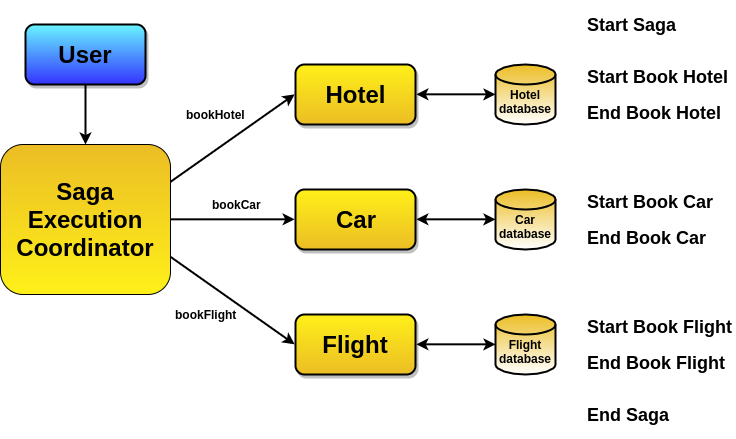
\includegraphics[height=60mm]{images/tripExample.png}
    \end{center}
    \caption{Example saga execution}
    \label{fig:tripExample}
\end{figure}

In this chapter, we will describe the saga processing as it is defined by the initial publication \cite{sagas_publ}, describe how the activities and compensations work in sagas, how the saga handles the failure recovery and present several modern frameworks that provide the support for the saga implementation.

\section{Activities}

An activity represents a local transaction that is a part of the saga. Each saga can be split into a sequence of activities in which each individually can be implemented with full ACID guarantees. When the activity completes, all results of the performed work are expected to be persisted in the durable storage. This means that the external observer may see the system in intermediate states of the saga execution, as well as that it may also introduce the system into an inconsistent state between the individual activity invocations.

The ability to commit a local transaction breaks the atomicity property as we no longer endure the atomic unit that the enclosing transaction represents. Furthermore, if distinct sagas may be executed in the system concurrently, the isolation (serializability) property is also violated. Although, intermediate saga states may introduce consistency contraventions, sagas guarantee that the state will become consistent after the saga completes. This principle is called an eventual consistency. It guarantees that even if partial execution may result into the inconsistent state, the system state will get consistent eventually -- there exist a point in future in which the system is consistent.

As the definition in the original paper by Garcia-Molina and Salem \cite{sagas_publ} allows local transactions to interleave, it prohibits any form of dependencies between them. This would imply that the participant cannot depend on results committed by any previous transaction in the saga sequence. However, in modern systems the sequential execution of local transactions is possible to implement in expense of an utilization of a single saga coordinator process throughout the entire sequential execution of this sequence. 

\section{Compensations}

Each activity in a saga needs to have an associated compensation transaction. The purpose of the compensating transaction is to semantically undo the work performed by the original transaction. This is not necessarily the contradictory action that puts the system into the same state as it was present before the activity began or generally the saga started. 

Imagine that the activity consists of the sending of an email. The saga compensation transaction cannot directly undo the email consignment. Instead it would send another email to the same destination which could explain why the previous action did fail. In this case, we can see that the system is in the state where it has two additional emails being send. However, the comprising system state is expected to be semantically consistent as both transaction and compensation have been defined by the participant. Therefore, the consistency guarantees must be ensured by individual participants at the activity level.

The compensating actions for the individual activities are expected to be idempotent. The main reason for this requirement is the saga failure and recovery management which in detail described in section \ref{sec:recovery-modes}.

It is important to keep in mind that even the compensating transactions may fail. There are several options of how the saga management system can handle such situations. The first option is to retry the compensating transaction again, but as the reason of the failure may still be valid, the system can get caught in an infinite retry loop. Another option is to provide a recovery block -- a separated block of code which would get executed in place of the primary compensation in case of failure. The last option, which is not elegant but it is practical, is the manual intervention. This is possible to implement due to the saga nature -- it does not hold any locks on resources it is being performed on. When the compensation handler is manually repaired, the saga can continue its execution where it has left off.

\section{Transactional properties}

In contrast to the traditional transaction approach, the Saga pattern relaxes some of the ACID properties to achieve availability and scalability with build-in failure management. As the saga commits each activity separately, this means that the updates of uncommitted long-lived transaction are immediately visible to other parallel activities \cite{trans_concept} which breaks the isolation property.

In practice, applications are not always fully restricted to all of the transaction guarantees, so the saga pattern is emerging as a real alternative to traditional ACID transactions\footnote{sagas utilize also the BASE model (basic availability, soft state and eventual consistency) which values the availability over the consistency of ACID}.

\section{Saga execution component and transaction log}

The saga execution component (SEC) is a process that is responsible for the saga management. It communicates with the transaction manager which manages activities included in the saga. Both of these components require a transaction log to record their respective interactions\footnote{it is convenient to share the transaction log between both components}. The saga execution component does not require  concurrency control because the saga activities can be interleaved.

The entries that may be written to the transaction log are usually associated with the saga or activity lifecycle. The saga log includes \texttt{start-saga} entry followed by one or more \texttt{start-activity} / \texttt{end-activity} entries and it is finished by the \texttt{end-saga}. Optionally, the transaction system may also provide an ability for users to cancel the saga execution with the \texttt{abort-saga} command. 

Each saga operation is channeled through the saga execution component and it is recorded in to the transaction log before any action may be taken. The transaction log can also contain any parameters associated with the saga execution.

\section{Recovery modes}
\label{sec:recovery-modes}

The saga paper \cite{sagas_publ} distinguishes two options to handle the failure that interrupts the saga. These two supported modes are backward and forward recovery.

\newlinepar{Backward recovery}

A backward recovery mode is the most common way of handling saga failure management as it was described in previous sections. It requires that all activities must define a compensation handler.

When the SEC component receives an \texttt{abort-saga} command in the backward recovery mode, it firstly abort the currently executed activity. Then for every previous activity in the reverse order of the original execution, it calls its respective compensation action. After the invocation of the compensation handler corresponding to the first activity is completed, the saga may end and the system is in semantically consistent state as it was before the saga began.

When the saga management system applies the backward recovery mode, the associated transaction log is also used to recover from the crashes of the saga coordinator. After the recovery, once all activities has been completed (committed or aborted), the saga coordinator determines the status of each saga execution by the investigation of transaction log entries. 

If the log contains only both \texttt{start-activity} and \texttt{end-activity} entries for the activities comprised in the saga,  than the execution is safe to continue with the next activity which has not been started. Another safe state is when the transaction log contains the \texttt{abort-saga} entry. In this case, it calls all compensation handlers for the referenced saga. This is possible due to the fact that all compensating actions are required to be idempotent.

The only unsafe state, that may be introduced after the saga coordinator recovers, is when the transaction log contains the \texttt{start-activity} entry without the corresponding \texttt{end-activity}. In this case, the saga coordinator selects the last successfully executed activity (contained in the transaction log) and invokes the compensation handler for this activity and all activities that have been executed before it.

As in the case of repetitive recovery for the same saga, the saga coordinator may call the corresponding compensation handlers repeatedly, the compensation actions are required to be idempotent. The original paper acknowledges that this constraint may be difficult to implement in some applications which is the reason for the introduction of the forward recovery mode discussed in the following section.

\newlinepar{Forward recovery}

For the use of the forward recovery mode, the transaction management requires that the saga itself is predefined and that the system is able to produce a check point. The check point represents a snapshot of the system state in the particular point in time into which the system can be always restored.

The pure forward recovery mode takes the checkpoint automatically at the beginning of each activity. Furthermore, it also disallows to abort the saga intermediate execution. This effectively eliminates the need to define any compensation actions. If the crash of the SEC occurs, it will abort the last executed activity and restart the saga from the last checkpoint. This approach effectively degrades the saga execution component to a basic persistent transaction executor, therefore loosing most of the saga benefits.

\hfill \break

In addition to modes defined above, it is also possible to combine these two approaches into the backward / forward recovery mode. In this mode, the transaction system takes checkpoints in predefined intervals which may be periodical or based on a different criteria (e. g. the activity complexity). In case of the SEC failure, the system performs the backward recovery to the last defined checkpoint and then continues the saga execution in forward recovery mode.

\section{Distributed sagas}

The notion of sagas can be naturally extended into distributed environments \cite{sagas_publ}. The saga pattern as an architectural pattern focuses on integrity, reliability, and quality, and it pertains to the communication patterns between services \cite{prac_ms}. This allows the saga definition in distributed systems to be redefined as a sequence of requests that are being placed on particular participants invocations. These requests may provide ACID guarantees, but this not restricted and it must ensured by individual participants. Similarly, each participant is also required to expose the idempotent compensating request which can semantically undo the request that is handled by this participant in the saga.

Analogously to the non-distributed systems, the distributed saga management also requires a transaction log which needs to be durable and distributed. The examples of distributed database providers include e.g. Cassandra, RethinkDB or Apache Ignite.

The saga execution coordinator (SEC) is spanned process across the participating services. This process manages and interprets the saga and it persists all processing information into the transaction log. The coordinator does not represent a single point of failure as it is allowed to fail. This is possible because the SEC process does not hold any state data, all of the saga state is held in the distributed log. The general example of the application model employing SEC is available in the figure \ref{fig:SEC}.

\begin{figure}
    \begin{center}
        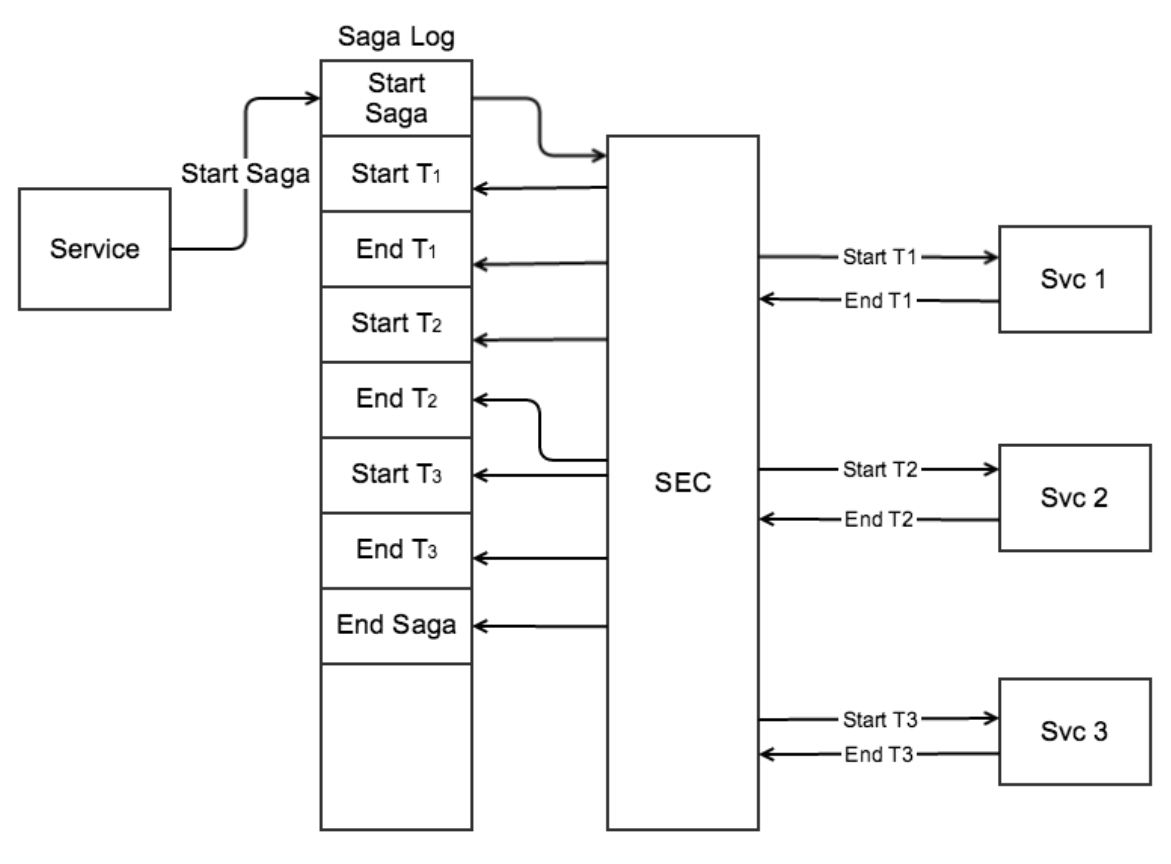
\includegraphics[height=70mm]{images/SEC.png}
    \end{center}
    \caption{Distributed saga example \cite{applying_saga_pattern}}
    \label{fig:SEC}
\end{figure}

As all of the above mentioned components are distributed, the saga management system needs to deal with a number of additional problems that are not present in the localized environment. The main problem is that the saga system is required to deal with network and participant failures that may happen between the remote invocations. There are four locations that can encounter the network failure -- writes for the beginning and end of the request to the transaction log and the request and response calls to the associated participant. This may introduce unnecessary saga aborts\footnote{if the SEC fails after it has written the \texttt{start-request} entry to the transaction log -- the recovery cannot determine whether the failure happened before the request, due to the network failure, or the participant response has been lost}, but generally the approaches from the non-distributed environment still apply.

\section{Current development support}

This section presents the current implementations of the saga pattern available for the enterprise use. The four explored frameworks are Axon \cite{axon_framework}, Eventuate Event Sourcing (ES) \cite{eventuate.io}, Eventuate Tram \cite{eventuate-tram} and Narayana Long Running Actions (LRA) \cite{narayana_lra}.

\subsection{Axon framework}

Axon is a lightweight Java framework that helps developers build scalable and extensible applications by addressing these concerns directly in the core architecture \cite{axon_framework}. It is composed on the top of the Command Query Responsibility Segregation (CQRS) pattern which is described in the Appendix \ref{sec:appendix-cqrs}.

The Axon framework is based upon the event processing including asynchronous message passing and event sourcing. To decouple the communication between system components, it employs the mechanisms of the asynchronous message buses. This allows to design components with well defined boundaries and therefore easy microservices development.

The CQRS architecture is directly embedded in the framework. Developers are controlling distinct CQRS components (aggregates, repositories, commands) by annotations. 

Axon supports two types of message buses -- the command bus and the event bus. This aligns with the CQRS pattern and allows to scale each part of the domain independently.

\newlinepar{Saga definition}

As the most of the Axon functionality, the easiest way to define sagas in an application is by annotations. The annotation \texttt{@Saga} marks the Java class as a saga implementation. In Axon sagas are a special type of event listeners. Each object instance of the saga class is responsible for the management of a single business transaction. This includes controlling the saga state information, execution and handling of the transaction (including start and stop) or performing the corresponding compensation actions.

All interaction with the saga class happens only by triggering of events. Event handlers in saga instances are annotated with the annotation \texttt{@SagaEventHandler}. 

To start a saga execution the framework needs to receive the event with the special event handler annotated with \texttt{@StartSaga}. By default, the new instance will be created only if the corresponding saga can not be found.

Ending of the saga can be defined by two means -- by the event or by the API call. If the ending event is used, than the conforming event handler needs to be annotated with the \texttt{@EndSaga} annotation. Alternatively, the conditional end of the saga can be signaled by the call to the \texttt{SagaLifecycle.end()} from some method inside the saga class.

As many instances of the saga class may exist at the same time, there is a need to publish events only to the saga for which they are intended. This is done by a definition of association values. The association value is a simple key-value pair where the key is a property present in the event which forms a connection to the saga instance. The \texttt{@SagaEventHandler} annotation contains a custom attribute called the \texttt{associationProperty} which denotes the key property in the incoming event. Axon also allows the definition of additional association values by a call to the \texttt{SagaLifecycle.associateWith(key, value)} and the \texttt{SagaLifecycle.removeAssociationWith(key, value)} inside any method of the saga class.

\subsection{Eventuate.io}

Eventuate is a platform for developing asynchronous microservices \cite{eventuate.io}. It focuses on the distributed data management allowing developers to focus on the business implementations. The platform consists of two products -- the Eventuate ES and the Evenetuate Tram. By the time of this writing, the Eventuate Tram was still in development and as it introduced the sophisticated saga processing to the platform, it is in detail described in the section \ref{sec:eventuate-tram}. This section presents the more general Eventuate ES product.

The Eventuate ES provides application with the programming model based on the event sourcing. Event sourcing is a mechanism that tracks all changes to the data model as a sequence of events stored in the event log. Every model change is appended to the log and the sequence can be anytime replayed to restore the application state. The event log can also serve as an auditing solution and provide temporal queries to track application previous states. Another advantage is that the events can be replayed to the failed service after it reconnects.


The ES project is also based on CQRS principles which allows natural employment of event sourcing capabilities for aggregate entities. It is provided in two versions -- as a service hosted on Amazon Web Services (AWS) or as open source local platform.

\newlinepar{Saga definition}

The saga processing of the Eventuate platform is handled by Eventuate Tram project and therefore the ES product do not support saga implementation directly. However, the example \textit{Eventuate service}, which is presented in the following chapter, is based exclusively on the Eventuate ES local platform providing the complete CQRS saga solution. It represents the user saga handling implementation not supported by the platform. 

\subsection{Eventuate Tram}
\label{sec:eventuate-tram}

The Eventuate Tram framework enables a Java/Spring application to send asynchronous messages as a part of a database transaction \cite{eventuate-tram}. It utilizes the traditional Java Database Connectivity (JDBC) and Java Persistence API (JPA) based persistence model to provide the transactional messaging. This enables microservices application to atomically update its state and to publish this information as a message or an event to other services.

The Eventuate ES platform builds the communication exchange on top of the event sourcing. Conversely, Tram provides three types of transactional messaging abstractions -- messaging, events and commands. The messages are sent trough dedicated named channels. The platform still supports the application development according to the CQRS pattern but it does not enforce it.

The Eventuate Tram Sagas is a framework that provides saga processing on top of the Eventuate Tram message passing. It introduced a very sophisticated saga model that allows to specify the saga definition as single point of reference. 

\newlinepar{Saga definition}

The saga is defined by the saga orchestrator -- the service responsible for the saga handling. It is identified as an implementation of the \texttt{io.eventuate.tram.sagas.orchestration.Saga} interface. The respective saga definition is represented as an instance of the class \texttt{io.eventuate.tram.sagas.orchestration.SagaDefinition}. This instance must be returned by the \texttt{Saga.getSagaDefinition} method. It can be specified with a simple fluent API that allows to define operations that should be executed when the saga fails, when it needs to invoke a participant or how to process participants compensations. 

The saga is defined as a sequence of steps specified by a simple Domain Specific Language (DSL) available in the \texttt{StepBuilder} class. Each step represents a local invocation, a remote participant invocation or the compensation definition. The last two return a participant builder which allows to additionally specify more actions that needs to be processed when the participant is invoked or the handler method which will be called when the participant responds.

\subsection{Narayana LRA}

Narayana Long Running Actions is a specification developed by the Narayana team in the collaboration with the Eclipse MicroProfile initiative \cite{saga-impl-comp}. It proposes a new API for the coordination of long running activities with the assurance of the globally consistent outcome and without any locking mechanisms.

The current reference implementation (RI) of the LRA specification is based on the Context and Dependency Injection (CDI) and Java API for RESTful Web services (JAX-RS) Java EE specifications. The communication is handled over HyperText Transfer Protocol (HTTP) by the Representational State Transfer (REST) protocol.

The LRA is utilizing an orchestration saga model. One node is selected as dedicated LRA coordinator that manages the saga processing. Its main responsibilities are the LRA initialization, participant enlisting and either completion or compensation of the saga. 

The coordinator can be a standalone service or it can be embedded within application service. For the second option, the coordinator communicates with the to the enclosing application by in-memory calls rather than REST.

The second model component defined in the LRA processing is the saga participant. This may be any service that is involved in the LRA. Each participant is required to provide at least two REST endpoints that serve as completion and compensation handlers respectively.

The execution of the LRA is started by the initiating service on the user request. The service calls the coordinator that in turn starts a new LRA and return its  unique identification to the initiating service. This id is used to enlist every participant within the saga. After the LRA id is received, the initiating service can optionally enlist itself and it continues the saga processing with other participants invocations where each call has to contain the acquired LRA id. When the participant is invoked, it will perform its work request, enlists itself within the received LRA and subsequently returns the processing outcome to the initiator. After all calls are completed, depending on the collected answers the initiating service calls the coordinator with one of the finalizing methods (\texttt{close} or \texttt{compensate}). The coordinator then performs the corresponding requested action for each of the enlisted participants.
 
\newlinepar{Saga Definition}

The LRA do not require users to specify the saga in any explicit way. The saga execution is handled by the initiating service. Narayana provides \texttt{io.narayana.lra.client.NarayanaLRAClient} class that allows users to perform basic requests for the coordinator operations. On the background, it calls the coordinator through its REST interface which users are also allowed to use directly. The \texttt{NarayanaLRAClient} is provided by the CDI dependency injection.

The participant is defined by annotations present on the JAX-RS resource class. The \texttt{@LRA} annotation declares the endpoint as saga participant. It takes as an argument the value of the transaction attribute which can have same values as for declarative transactions presented in section \ref{sec:decl-tran-model}. This JAX-RS endpoint must also expect the \texttt{NarayanaLRAClient.LRA\_HTTP\_HEADER} header parameter that contains the coordinator address and the LRA identification. Depending on the value of the transaction attribute, the participant can be automatically enlisted to the saga without any intervention.

The participant is also required to expose at least two additional endpoints that handle the end phases of the execution. The specification where these endpoints are present needs to be propagated to the coordinator. If not specified, by default the coordinator expects them on the request endpoint with respective suffixes (\texttt{/complete} or \texttt{/compensate}). The participant is also allowed to specify these methods with annotations (\texttt{@Complete} or \texttt{@Compensate}) that define the handler outside of the JAX-RS context for the possible future implementations. The complete and compensate are required but not the only possible endpoints that the participant can expose. Other potential values are status, forget and leave where each has its respective handling inclinations to the LRA participant processing \cite{narayana_lra}.


\clearpage
\chapter{Saga implementations comparison example}

As a part of the investigation of the each discussed framework from the previous chapter, I created a sample application simulating the saga utilization. The main goal of this quickstart projects is to compare the base attributes of the investigated saga solution frameworks. This includes the comparison of the development model, microservices feasibility, maintainability, scalability, performance and the applicability of the reactive principles within the saga execution. The examples created for this thesis may be considered as artifacts of the one iteration of the design science research \cite{design_science}.

The application represents a backend processing for orders with a simple REST\footnote{Representational State Transfer} user interface. Users are also allowed to query persisted information through the defined microservices APIs available in appendix \ref{sec:appendixAPI}.

All examples are based on the microservices pattern. As every framework is suitable for the use in different environments, each example is achieving the same goal through the different portfolio of technologies. The exact mechanisms used is individual projects will be discussed in more detail in their respective sections.

\section{Common scenario}

A user is able to create the order by a REST call to the dedicated endpoint of the \texttt{order-service} microservice. The request must provide a product information JSON\footnote{JavaScript object notation} containing a product id, a commentary and a price. For the simplicity reasons, the order always consists only of the single product. The figure \ref{fig:inputJson} shows the example of the input JSON format for the product data. The complete REST API\footnote{Application programming interface} for each individual example is provided in the Appendix \ref{sec:appendixAPI}.

\begin{figure}
    \begin{center}
        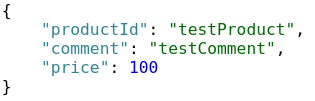
\includegraphics[height=30mm]{images/productInfoJSON.png}
    \end{center}
    \caption{Product Information example JSON}
    \label{fig:inputJson}
\end{figure}

The setup of each example is described in detail in their respective repositories. Generally, each service is a standalone Java application that must run in a separated terminal instance by default located on the local computer address (localhost). Except for the LRA example, all examples are also able to run on the Docker\cite{docker} platform using the Docker compose project\cite{docker_compose}.

Every saga invocation is asynchronous - the REST call for the order request directly returns an order identification number in the response. All of the following interactions are documented in individual services by messages that are logged by the underlying platform. The overall saga process can be examined in the \texttt{order-service} or in the case of LRA in the \texttt{api-gateway} modules.

Users are also allowed to query the persisted saga information (orders, shipments and invoices) by the respective REST endpoints described in the Appendix \ref{sec:appendixAPI}. For the CQRS based examples this information is available at the \texttt{query-service} microservice, otherwise each service is expected to be responsible for maintaining its individual persistence solution which corresponds with the microservices pattern definition.

\section{The saga model}

The saga pattern used in this application is able to create orders. The order saga consists of three parts -- the production of a shipping and an invoice information and if both invocations are successful, the actual order creation. If any part of the processing fails, the whole progress is expected to be undone. For instance, if the shipment is successfully created but the invoice assembly is not able to be confirmed, the persisted shipment information as well as the order must be canceled (also optionally notifying the user that the order cannot be created). The graphical representation of the saga progress is available in the figure 6.2.

\begin{figure}
    \begin{center}
        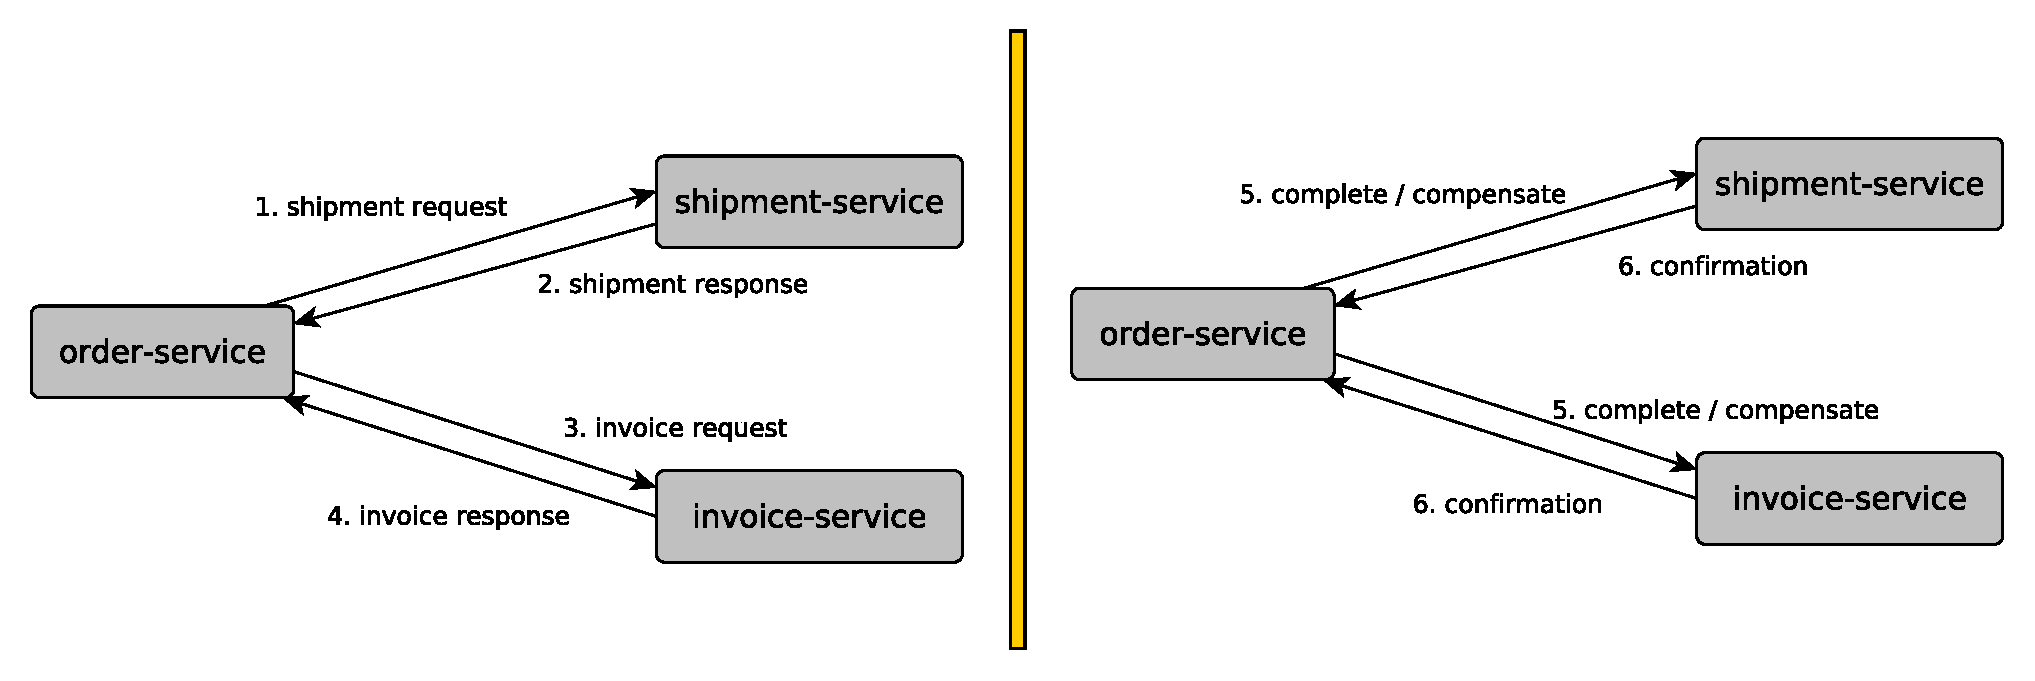
\includegraphics[height=40mm]{images/sagaModel.pdf}
    \end{center}
    \caption{The saga model}
\end{figure}

Every application is able to demonstrate three testing scenarios: the valid pass, the shipment failure and the invoice failure. In the valid scenario after the order is requested, the saga propagation invokes requests for the shipment and the invoice. If the connection between services is stable, both participants successfully return a stub answer and the order is completed. 

As most of the applied platforms invoke participants in the synchronous way, we distinguish separated member failures of the shipment or invoice. The shipment failure simulates the termination of saga without the full request coverage. This means that the compensations are distributed to all services including the \texttt{invoice-service} which has not received the work request for the order being processed yet. The scenario demonstrates the need of microservices to be able to react to the requests which are not associated with any saga which means actively keeping track of the sagas being currently executed. 

The invoice failure scenario on the other hand validates that the saga compensations are executed on all participating services as the shipment is already expected to be completed. Generally, the saga pattern assumes that the compensations of the participants are called in the reverse order of the invocations because of the possible dependencies between them.

To initiate the failures scenarios in examples both \texttt{shipment-service} and \texttt{invoice-service} are equipped with injected failure conditions. To invoke the failure the quickstarts expect a product information containing a specialized product identification: \texttt{fail-shipment} or \texttt{fail-invoice} respectively. 

The graphical representation in form of the sequence diagrams for corresponding scenarios is available in the Appendix \ref{sec:appendix-scenarios}.

\section{Axon service}

As it was stated in the previous chapter, the Axon framework is based upon the CQRS principles. Because of this nature, it would be difficult not to follow this pattern. The individual services contain separated aggregates\footnote{for the definition of aggregate please refer to the Appendix \ref{sec:appendix-cqrs}} each processing its respective commands and producing various events. Any inter-service interaction is restricted to the use of the command and event buses.

\subsection{Platform}

Axon service is a Java Spring Boot \cite{spring_boot} microservices application. Each service is fully separated and independent Maven  project \cite{maven}. Every project is standalone runnable application (fat java archive (jar)) as the Spring Boot does not use any underlying platform to run microservices.

As a CQRS based quickstart, Axon service uses two different and separated communication channels to exchange information between services: the command bus and the event bus. By default, the Axon framework reduce both channels to one JVM therefore one microservice. However, developers are also able to specify several specialized ways of the configuration to distribute messages between different services which is used in this Axon quickstart.

The quickstart uses a motion of the distributed command bus which is based upon a different approach then the one used in the traditional single JVM Axon applications. The distributed command bus forms a bridge between separated command bus implementations to transfer commands between different JVMs \cite{axon_framework_reference_guide}. Its main responsibility is the selection of the communication protocol and the choice of the target destination for each incoming command. 

Axon provides two options for connecting different services through the distributed command bus -- \texttt{JGroups Connector} and \texttt{Spring Cloud Connector}. The one used in this quickstart is the Spring Cloud method. The underlying implementation employed in this quickstart is based on the Netflix Eureka Discovery and Eureka Server combination \cite{service_registration}. Each business service as a part of its initialization registers itself with the  \texttt{registration-server} service which function as the Eureka server. Axon is then able to redirect commands to the right service chosen by the value of parameters in the command class annotated by the \texttt{@TargetAggregateIdentifier} annotation.

For the distribution of the event bus Axon service uses an external messaging system based on the Spring Advanced Message Queuing Protocol (AMQP) protocol called RabbitMQ message broker \cite{rabbitmq}. The quickstart uses separated messaging queue for each business service and one separated queue for the \texttt{query-service} microservice which is subscribed to all of the processing events. Axon platform provides the direct support for the AMQP so no specific handling of the produced events is required -- Axon automatically distributes events to all connected queues.

It is worth mentioning that both the Spring Cloud and the RabbitMQ message broker are required external providers that need to be started before the deployment of the business services. Unfortunately, by the time of this writing there is no way to distribute commands or events directly in the Axon platform.

\subsection{Project structure}

The application is composed of five microservices -- the  \texttt{order-service}, the \texttt{shipment-service}, the \texttt{invoice-service}, the \texttt{query-service} and the \texttt{registration-server}. Furthermore it also contains a separated project \texttt{service-model} which serves as a support library for the other microservices.

As it was stated in the previous section \texttt{registration-server} microservice is a Spring Boot application which function as a Netflix Eureka server. Other business services act as clients for this server, therefore it is required that this service is initialized by the time they try to register.

The \texttt{order-service} project is a business microservice responsible for the saga handling. It contains the logic for the order request, the saga initiation and the saga compensation.

Both \texttt{shipment-service} and \texttt{invoice-service} are business services functioning only as the saga participants. Their only obligation is to provide their respective computations.

The \texttt{query-service} is a specific microservice included for the purposes of the CQRS pattern. It collects the information of the prepared orders, shipments and invoices and provides an external APIs for the querying of these resources. 

Finally, the \texttt{service-model} is a Kotlin and Java Maven application providing the core API for the commands and events used by various business services. This is required as all classes must match in order for particular handlers to be invoked. Furthermore, it also provides common utilities and the logging support. It is mandatory to include this project on the classpath of the every other service.

\subsection{Problems}

\newlinepar{Maintenance of the saga structure}

The one substantial problem the saga processing in Axon has is the missing structure of the internal life cycle of the saga. Axon only provides ways to indicate the start and the stop of the saga. The actual invocation of the participants, collecting of the responses and handling of the compensations is up to developer as the only way of communication with the saga is through events.

In this application the \texttt{OrderManagementSaga} contains two internal classes -- \texttt{OrderProcessing} and \texttt{OrderCompensationProcessing} which are responsible for keeping track of the saga execution and compensation respectively. As production ready sagas can be expected to run in a number of days, this can quickly become the bottleneck of the saga maintenance.

\newlinepar{Distribution of events to sagas}

Another encountered problem is that by the time of this writing Axon does not provide an easy method for the configuration of the different event bus for saga events than is the one that is used by default. The \texttt{@Saga} annotation is preconfigured with the value of the local event bus which is not allowed to be changed. The workaround is to manually register a custom saga manager which is not straightforward from the user perspective when the saga needs to be distributed through different JVMs.

\newlinepar{AMQP usage with sagas}

When the distributed event bus is processing events from an AMQP queue which the saga class is listening to, the framework does not deliver events correctly to the attached handlers. This may be caused by the incorrect configuration from the previous problem. The workaround used in the quickstart is to artificially wait 1000 milliseconds before delivering the event from the queue to the framework.

\newlinepar{CQRS restrictions}

As CQRS is a pattern that manages the domain formation of the application, Axon can place a hard requirements for the projects that do not follow the CQRS domain separation. Like it was already presented, sagas in Axon are only a specialized type of the event listener. The only way Axon produces events is trough an interaction with the aggregate instance - events are produced purely as a response to the received command. Therefore the use of Axon sagas in not CQRS environment may be too restrictive for an implementation.

\subsection{Technology}

This example contains a set of Spring Boot applications which can be run directly from the command line. Additionally, it also contains docker and docker-compose configuration to ease the development and deployment operations. In this section we focus on the Spring platform, the Docker description is provided in the section \ref{sec:docker}.

\newlinepar{Spring Boot}
\label{sec:spring-boot}

Spring Boot is a framework built on top of the Spring Framework \cite{spring_ms}. Its main focus is on the creation of standalone runnable applications that are easily employed in microservices architectures. It favors convention over configuration to allow the usage of Spring features with a little of the Spring configuration \cite{spring_boot}.

The Spring Boot platform is composed into aggregate modules known as \textit{starters}. The starter is a dependency descriptor which contains dependencies that are required to provide some functionality to the application. In order to use Spring Boot, the \texttt{spring-boot-starter} core module must be incorporated. Other useful modules, for instance, \texttt{spring-boot-starter-web} or \texttt{spring-boot-starter-data-jpa} can be provided to support the microservice adoption. Starters can be packaged with the application using Maven or Gradle build configurations.

Another responsibility of this framework is the packaging of the application. The preferable way for the microservice is to create an executable fat Java archive (jar) which contains all of the application dependencies. The application can then be simply excuted by a \texttt{java -jar} command.

A spring Boot microservice must fulfill two requirements -- it must follow a Maven layout convention and it must provide an entry point. This can be any class annotated with the \texttt{@EnableAutoConfiguration} annotation that starts the Spring Boot context.

Spring provides various ways for exposing available services. Registration servers like Eureka or Consul which are integrated within the Spring cloud \cite{spring_cloud} can be used as the service discovery mechanisms. For a manual approach, the microservices functionality can be exposed through the RESTful API.



\section{Eventuate service}

Similarly to Axon, Eventuate service is also based on the event sourcing and the CQRS pattern. For this reason, the business execution is managed in the aggregates which correspond to the respective microservices projects. The communication is as a result restricted to the command processing and the event appliance.

This quickstart represents the pure CQRS approach to the saga processing. This means that the whole saga implementation is created by the developer using the platform only for the event and command distribution. For this reason, the Eventuate service is more complex than any other quickstart but for the example purposes, it distinctively demonstrates how sophisticated is the saga administration provided by all remaining platforms.

\subsection{Platform}
\label{sec:eventuate-platform}

Eventuate service is a microservices application consisting of a set of Spring Boot \cite{spring_boot} business services, one backing module and a number of support services provided by the Eventuate platform. In this section, we will focus on the Eventuate platform and the services it provides, the business part of the application is described in the following section.

This quickstart is established as a Eventuate Local version of the platform. This means that it uses underlying SQL database for the event persistence and the Kafka streaming platform for the event distribution. Eventuate Local provides five services used by the quickstart that are managed by the platform, namely Apache Zookeeper, Apache Kafka, MySQL database, the change data capture component and the Eventuate console service. The example employs these services as a Docker images included in the provided docker-compose configuration.

\newlinepar{Apache Zookeeper service}

Apache Zookeeper is an open-source project which enables highly reliable distributed coordination \cite{apache_zookeeper}. It maintains a centralized service which supervise various functionalities like handling of the configuration information, synchronization, naming or grouping. The Eventuate Local platform provides its own Docker image tagged as \texttt{eventuateio/eventuateio-local-zookeeper}.

\newlinepar{Apache Kafka service}

The Apache Kafka streaming platform is the service which is responsible for the administration of subscription and publishing mechanisms controlling the event processing for the business microservices. As it is based on the Streams API it allows the platform to react to events in real time. Eventuate manipulates Kafka as the notification service for the event propagation. Eventuate ships its own Kafka version in the \texttt{eventuateio/eventuateio-local-kafka} docker image.

\newlinepar{MySQL database service}

The SQL database used in this application for the event persistence is the MySQL open-source database which is currently the only database supported by the platform. The Eventuate Local maintains two tables -- \texttt{EVENTS} and \texttt{ENTITIES}. This database serves also as a transaction log maintained as a mean for the event sourcing. The containerized version is located under \texttt{eventuateio/eventuateio-local-mysql} tag.

\newlinepar{CDC service}

This service represents the change data capture (CDC) component. The CDC service has two main responsibilities -- it follows the transaction log and it publishes each event which is inserted into the \texttt{EVENTS} table to the Kafka topic that corresponds to the aggregate for which the event is intended. Eventutate Local supports two options of the execution of the CDC -- internally in each business service or as a standalone application. This quickstart applies the Eventuate CDC service \texttt{eventuateio/eventuateio-local-cdc-service} as a standalone Docker container.

\newlinepar{Eventuate console}

The last support service is the \texttt{consoleserver}. It provides a simple interface for accessing the information about created aggregate types and the event log. The supplied Docker container image is the \texttt{eventuateio/eventuateio-local-console}.


\subsection{Project structure}

This section describes the set of services composing the business side of the application. This set contains four services that cover the saga execution and data processing (\texttt{order-service}, \texttt{shipment-service}, \texttt{invoice-service} and \texttt{query-service}), one service (\texttt{mongodb}) representing the persistent storage and one additional support module (\texttt{service-model}).

All of the business services are a Spring Boot applications based on the Gradle \cite{gradle} build system. Each microservice is represented as a independent module capable of being separately built and deployed. Even if Spring Boot projects can be executed directly from the command line as ordinary Java applications, this quickstart leverages the Docker approach of the Eventuate Local platform and containerize all of its services.

To connect to the Eventuate platform each service defines a set of environment variables that are leveraged in their Spring Boot configuration. This information includes the connection and authentication details for the MySQL database, the CDC component and the connection URLs\footnote{Uniform Resource Locator} for the Kafka and the Zookeeper services. These variables are specified in the container specification for each individual business service in the \texttt{docker-compose.yml} file.

The actual saga execution is managed in the \texttt{order-service} microservice. The saga realization implementation is contained in three classes -- the \texttt{OrderSagaAggregate}, the \texttt{SagaEventSubscriber} and the \texttt{OrderSagaService}. The first class is an ordinary CQRS aggregate that handles the commands for the saga initialization and the participants outcomes. Conversely, the latter one is the event processor listening for the events produced by the aggregate which is basically a wrapper around the \texttt{OrderSagaService} - the class responsible for the remote REST calls to the other services and the command dispatching for the \texttt{OrderSagaAggregate}. The usage of the separated event listener is required because Eventuate does not allow aggregates to be declared as Spring components. The reason of this defect is described in more detail in the following section.

Except for the normal order API, the \texttt{order-service} also provides a management API for the participants to be able to share the information about their processing. This endpoints are hardcoded in the application which may not be acceptable for a production realization.

The \texttt{shipment-service} and the \texttt{invoice-service} both contain a simple aggregate together with its associated event listener which control the participant interaction with the saga. Each service also accommodate the REST endpoint for the saga request and its possible compensation.

Similarly to Axon service, the \texttt{service-model} project acts as a support library for other services. It contains a core API for each business service which needs to be shared and the utilization classes.

The last business microservice is the \texttt{query-service}. It performs as a response service providing the information about persisted orders, shipmetns and invoices. It contains an event listener for each designated microservice which in turn preserve the achieved information in the Mongo NoSQL database. This service also provides a simple Swagger interface to ease the user application interaction.

\subsection{Problems}

\newlinepar{Complexity}

As this project represents a plain CQRS based example it completely demonstrates the background process required for the saga execution. Therefore the complexity of this quickstart may appear more critical than in other projects as the background saga execution often contains many optimizations.

The first complexity problem is that the project contains a great number of the command and event classes. This is required as aggregate classes are only able to consume commands and produce events. For that reason,  the communication between components often demands a few additional steps.

The full saga administration is handled by the project from the very beginning. That covers the support of starting, stopping and following the saga execution as well as saga compensations. The restrictions placed by the CQRS pattern furthermore put additional requirements on the saga processing which may not be demanded by other frameworks. Before the Eventuate Tram framework, the Eventuate platform did not provide any saga support.

This quickstart uses the REST architectural style for the remote communication between services. Even if all of microservices are connected to the same MySQL database, they cannot directly propagate commands between each other. This is due to the way Eventuate dispatches commands through the aggregate repository. The aggregate repository represents the database table that is restricted to one aggregate and consequently, it needs to be injected by the platform. For this reason, it needs to declare the target aggregate class and the command type. The sharing of the aggregate class may be very restrictive, especially for microservices applications.

\newlinepar{Aggregate instantiation}

The Eventuate framework creates the instances of the aggregate classes by a call to the default constructor. This effectively prohibits the use of aggregate instance managed by the underlying server container. 

For this reason, each aggregate in this project is separated into two classes -- the actual aggregate responsible for the command processing and the event subscriber instance managing the incoming events. The  aggregate class is required to extend the \texttt{ReflectiveMutableCommand\\ProcessingAggregate} specifying the type of the command interface which allows the classpath instantiation. The event listener is defined by the \texttt{@EventSubscriber} annotation which permits it to be constructed as a Spring container component for the dependency injection employment. 

This restriction is seconded by the rule stating that each produced event from the aggregate's command processing method must also be applied by the different method of the same aggregate. This limitation exists because of the event sourcing feature providing the ability to replay already executed commands to reconstruct the aggregate's state in the case of failure. The aggregate then may contain unnecessary empty methods as the saga also requires the propagation of the information to different components (e. g. the REST controller).


\newlinepar{Event entity specification}

As well as the command type, Eventuate also requires the definition of the event type each aggregate is able to produce. The event class is defined as a value of the \texttt{entity} attribute of the \texttt{@EventEntity} annotation. This annotation is usually placed on the event interface which implementation represents produced events.

The problem rises when the events needs to be shared between several modules. This is a common requirement as the CQRS pattern requires the query domain to be separated. The event interfaces are therefore included in the common library module as the \texttt{service-model} used in this project. The hard coded information of the full name of the aggregate class used in the \texttt{@EventEntity} annotation then may become hard to maintain.

\newlinepar{Platform structure}

The platform structure places the obligation on each developed microservice to conduct with the connecting specification. This means that every service must provide linking information for the Eventuate platform services described in the previous section, namely MySql database, Apache Kafka, Apache Zookeeper and CDC component. This information is manually replicated in each service (restricted to system properties) and therefore predisposed to errors.

\hfill \break

In the end it is worth mentioning that as the Eventuate service is the pure CQRS saga example it has a few problems which has been reduced or removed in the later Eventuate Tram implementation that is in detail described in the following section. 

\subsection{Technology}
\label{sec:eventuate-technology}

This section provides a detailed view of the Docker platform, for the description of Spring Boot microservices please refer to the section \ref{sec:spring-boot}.

\newlinepar{Docker}
\label{sec:docker}

Docker is an open source container platform designed to make it easier to build, secure and manage the widest array of application from development to production both on premises and in the cloud \cite{docker}. Docker containers allow applications to run on top of the kernel services provided by the hosting system which considerably effects the application performance. However, it still builds containers on top of the generalized interface which warrants straightforward portability between different machines.

A container image is a lightweight, stand-alone, executable package of a piece of software that includes everything needed to run it -- code, runtime, system tools, libraries or settings \cite{docker}. All docker containers that run on the same machine share the kernel services of the host. The images are build on the concept of layers. The layer provides an abstraction to share common filesystems, configuration and other data that can be reused by several docker containers.

Containers isolate applications from the operating system their running on and also provide the separation from other docker containers running concurrently on the same computer. Instead of virtual machines which provide similar functionality, Docker virtualizes the operating system not the hardware. Docker provides abstraction at the application level.

Docker as a tool is targeted for simple utilization. It provides an unified environment for both developers and administrators supporting the DevOps (development and operations) practices. Particularly, developers profit from portable code that is able to run on any operating platform supporting Docker, while operations gain visibility and management services from comprehensive control panel covering all containerized applications.

\newlinepar{Docker compose}

Docker compose is a tool for the defining and running multi-container Docker applications \cite{docker_compose}. It allows to specify configuration for several containers as YAML file that can be passed as an argument to the command line tool to run all services with a single command.

The YAML configuration includes the same options that are available as a switches to native Docker commands. Additionally, it also provides functionality to orchestrate the specified services once they are started through the \texttt{docker-compose} command line utility. These functions include the network definition which allows easy addressing and the location transparency of the employed containers, the preservation of the container volumes, recreation of only changed containers or the specification of environment variables directly in the configuration file. 

Docker compose represents a simple way to provide container automation that may ease the development and support of the continuous delivery (CD) and integration (CI) pipelines.

\section{Eventuate Sagas}

The Eventuate Sagas quickstart is based on the new Eventuate Tram framework. This framework provides several solution to problems with saga management that are present in the Eventuate platform.

\subsection{Platform}

Similarly to the full Eventuate distribution, the Eventuate Tram establishes four services that form the Tram platform: Apache Zookeeper, Apache Kafka, MySQL database and CDC component. The fifth Console service is not present as the platform does not provide this functionality by the time of this writing. As all mentioned services represent the same functionality as they are responsible for in the full Eventuate platform, the individual descriptions of each service is defined in detail in the section \ref{sec:eventuate-platform}.  

All services are deployed by the \texttt{docker-compose} configuration distributed with the framework. This setup is based on the same Eventuate docker images for \texttt{zookeeper} and \texttt{kafka} services, and with \texttt{mysql} and \texttt{cdcservice} redefined by Tram.

\subsection{Project structure}

As Eventuate Tram does not restrict its services to the CQRS pattern, this project, in contrast to Eventutate service, contains only three business microservices and one support module. Every service is configured in the similar way as for the full platform containing the references and authentication details for the MySQL database, Kafka framework and Apache Zookeeper service. The quickstart is distributed with the predefined \texttt{docker-compose} configuration file that enables one command start up of all services.

The last service which is not required for the saga execution and handling is the \texttt{mongodb} NoSQL server. This service is present only for the demonstration purposes to allow the data retrieval on individual business services from different storage than the one that is used by the Eventuate platform.

The first microservice \texttt{order-service} is responsible for the order requests and saga processing. It also provides the ability to query persisted orders from the remote Mongo database.

The most important element in the \texttt{order-service} is the saga definition that is located in the \texttt{OrderSaga} class. This definition uses the declarative approach with the fluent API to denote the saga in steps of execution. Every step declares a handler method to be invoked when the step is reached by a reference to private methods in this class.

The step provides an ability to advance the saga execution in three ways -- by invoking of the local function, by a call to the remote participant or by the definition of the compensation method for the saga. Furthermore, the participant is able to define individual actions that comprise its engagement in the saga, the compensation handler and several reply handlers that are distinguished by the data object class that is received in the reply. This definition provides a simple in one place saga specification which is suitable for easier maintenance and distribution. This declarative approach provides many advantages that will be detailed in the following chapter.

The last two business services that contribute to the saga execution are \texttt{shipment-service} and \texttt{invoice-service}. Both of these microservices define several command handler methods associated with the channel that is dedicated to the service. 

The channel is a main communication mechanism used in Eventuate Tram. It is denoted by a string name that needs to be specified in the command message as a target destination. The definition of channel associates commands that it is able to receive with command handling methods that are invoked when the corresponding commands are delivered. The command handler returns a \texttt{Message} object identifying the outcome of the invocation. The failure outcome of any participant will immediately result in the saga compensation.

Both services are also connected to the Mongo database server in order to provide the browsing of the created shipments or invoices respectively.

In conclusion, Tram remarkably simplified the Eventuate platform for the usage of sagas. Most importantly, it introduced a simple fluent API for the saga definition and the loss of CQRS restrictions. Altogether, Tram platform makes a suitable saga solution for microservices based environment.

\subsection{Problems}

\newlinepar{Destination identification}

The destination channels in Tram are distinguished by a simple string which may cause problems in the case of name conflicts. Currently, the choice of the handler to be invoked depends on two resources -- the name of the channel and the command dispatcher id. When both strings match the same destination even in different services, the platform delivers the commands between handlers in random fashion which may become a complex issue in larger projects.

\newlinepar{Command handlers}

Handler methods that are referenced in the definition are restricted to the communication model provided by the platform. This allows a single command to be sent to the required destination. Unfortunately, platform does not allow the saga to perform any other operation without the participant invocation which may lead to unnecessary empty commands and channels declarations. 

Similarly, the saga may need to interact with the same participant in several different commands. This may cause problems with definitions of compensation and reply handlers as the developer needs to mind the logical grouping of participant invocations.

\subsection{Technology}

Eventuate Tram is based on the same microservices platform structure as standard Eventuate framework and therefore the same technology. For the description of the technology employed in this quickstart please refer to the section \ref{sec:eventuate-technology}.

\section{LRA service}

The LRA service is the first example which differs from previous quickstarts as it does not restrict its services to any particular conventions. Individual services are connected through the exposed REST routes.

\subsection{Platform}

This quickstart is composed as a set of WildFly Swarm microservices applications. Every microservice is designed to be easily deployed to the OpenShift container application platform provided by Red Hat, Inc. \cite{openshift} Both of these platforms are in detail described in the following technology section.

Each service uses the \texttt{fabric8-maven-plugin} for the build and the deployment to the OpenShift platform. This plugin provides a straightforward way of declaring the necessary configuration information the platform requires to orchestrate the service according to the user demands. This project applies the source to image (S2I) toolkit that builds imminent Docker images which can by immediately deployed to the OpenShift. 

As it was already presented in the previous chapter, Narayana's long running actions are not composed as a platform, but rather as a standalone coordination service. This project employs the standalone Narayana LRA coordinator service which is constructed as a WildFly Swarm microservice called \texttt{lra-coordinator}. 

All other traditional microservices requirements are handled by the OpenShift platform. This covers service discovery and location transparency, monitoring, logging, resiliency and health checking (failure discovery) which is why this configuration is not included in example services.


\subsection{Project structure}

This project consists of five WildFly Swarm microservices and one support module. Each service is designed and configured with the \texttt{fabric8-maven-plugin} providing simple deployment to the OpenShift platform. Additionally, services contain a customized Dockerfile specifying environment properties and the target Swarm uberjar file which is used for the source-to-image (S2I) builds in OpenShift.

The support library project is called the \texttt{service-model}. This module is rosponsible for the definition of the LRA information, the specification of the exchanged JSON data formats, the description of the communication model used in other services and the administration of common utilities.

The \texttt{LRADefinition} class denotes the JSON format of the LRA representation. It presents a simplified version of the LRA capabilities for the example purposes. The definition includes only required attributes -- the name of the LRA, a list of individual actions that form the LRA and the unspecified object containing the user defined information associated with the LRA. The example LRA definition JSON format is available in the figure \ref{fig:lra-json}.

\begin{figure}[h]
    \begin{center}
        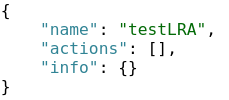
\includegraphics[height=30mm]{images/LRADefinition.png}
    \end{center}
    \caption{LRA definition example JSON}
    \label{fig:lra-json}
\end{figure}

The individual actions that compose the LRA are incident to the pattern services in this quickstart use for the communication. The information exchange is based upon the REST architectural style which expects that services adhere to predefined endpoint rules. 

The action definition consists of the name, the action type and the service for which the invocation is intended. The \texttt{service-model} project contains both \texttt{ActionType} and \texttt{Service} enumerations that denote possible values. The example action JSON is included in the figure \ref{fig:action-json}.

\begin{figure}[h]
    \begin{center}
        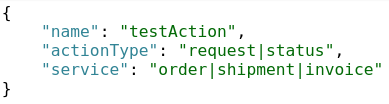
\includegraphics[height=30mm]{images/actionJSON.png}
    \end{center}
    \caption{Action example JSON}
    \label{fig:action-json}
\end{figure}

The actual deployable microservices project consists of five services -- \texttt{api-gateway}, \texttt{order-service}, \texttt{shipment-service}, \texttt{invoice-service} and \texttt{lra-coordinator}. Every service is configured with the addresses of other services as they reflect the OpenShift/Kubernetes application names. All of exposed APIs are defined in the Appendix \ref{sec:appendixAPI}.

The services that provide the LRA execution capabilities are the \texttt{order-service}, the \texttt{shipment-service} and the \texttt{invoice-service}. Every service provides a simple computation that contributes to the LRA realization. Additionally, \texttt{order-service} also provides a user invocation endpoint that can initiate the LRA. As all three services are eventually subscribed to the LRA, they all provide REST endpoints annotated by the LRA annotations for the completion and compensation invocations. Each service is configured with an in-memory H2 SQL database for the data persistence.

The \texttt{lra-coordinator} project is provided by the Narayana framework. Although the LRA specification does not require the application of the REST architectural style, the \texttt{lra-coordinator} operates a set of REST endpoints that maintain the start of the LRA, gathering the information about active and recovering LRAs, the management of the nested LRAs and the ability of participants to join (enlist in) or leave the LRA. Narayana distributes this project already as a WildFly Swarm distribution. but for the investigation purposes, this quickstart still builds it as a part of the S2I deployment.

Even if the \texttt{lra-coordinator} presents the REST endpoints for the LRA management, this quickstart invokes the coordinator by the client module provided by Narayana. The \texttt{lra-client} dependency provides the \texttt{LRAClient} class that is configured with the coordinator location and serves as a proxy separating the user from the actual REST invocations. This class is defined as a CDI bean to enable simple use through the dependency injection. The participant enlisting and invocations are defined by annotations present in the \texttt{io.narayana.lra.annotation} package.

The last service is the \texttt{api-gateway}. This module functions as an interface that makes the LRA execution transparent for the invoking services. The current state of the Narayana handling of LRA requests will be described in the following section.

The \texttt{api-gateway} uses the LRA and action definition classes from the \texttt{service-module} to handle the LRA processing on the behalf of the initiating service. It exposes a REST interface that consumes the LRA definition JSON.

The actual LRA execution is managed in the \texttt{LRAExecutor} class. This class provides one public method \texttt{processLRA(LRADefinition lraDefinition) : void} that is responsible for starting and performing of the LRA, collecting the participants results and closing or compensating of the LRA. This method processes the LRA asynchronously -- each execution is propagated to the new thread from the cached thread pool defined by the executor service present in the \texttt{LRAExecutor} class.

As this module was designed for this particular LRA scenario, it is configured to execute the LRA actions (order, shipment and invoice requests) independently and in parallel. It collects the result of each action and eventually closes or cancels the LRA with methods provided by the \texttt{LRAClient}. Certainly, this is an area which could be in a more general execution module further extended with e.g. the sequential configuration or the LRA nesting.

\subsection{Problems}

The Narayana Long running actions are a very efficient development model for the microservices applications. Although, it mainly aims for the compatibility with the MicroProfile specification (REST and CDI), it does not restrict microservices to essentially any other particular implementation restrictions. Even if the MicroProfile is restricted to REST invocations, Narayana LRA specification does not require the usage this architectural style for the communication with the coordinator. However, the only implementation that is currently available is based on REST, but it certainly can be extended to other communication protocols in the future.

The only problem that may occur in the current implementation is that the LRA framework provides only coordination and management capabilities, it does not handle the saga structuring and execution. Extraction of these capabilities directly to the LRA processing would be certainly applicable in many common specifically reactive applications use cases which can ease the development and orchestration of the saga execution. 

In the LRA service is this problem addressed by the \texttt{api-gateway} service which functions as a proxy for the \texttt{lra-coordinator} that handles the saga execution. This approach does not effect the Narayana LRA management. The only change from the traditional processing is that series of LRA actions are performed by the \texttt{api-gateway} instead of the initiating service. This allows the service to be immediately available for the subsequent user requests and to scale the LRA processing independently from the application services that utilize the saga actions execution.

\subsection{Technology}

This section describes technologies included in the LRA example -- the WildFly Swarm project as underlying microservices provider and the OpenShift and Kubernetes containerization platforms as the quickstart has been designed for the deployment to these environments.

\newlinepar{WildFly Swarm}

WildFly Swarm is the Red Hat microservices initiative designed to enable deconstructing the WildFly application server and pasting just enough of it back together with the application to create a self-contained executable jar \cite{gupta_2018}. 

The traditional Java Enterprise Edition (EE) approach follows the development of the application and its successive deployment to the application server which includes necessary dependencies which the application requires to run. On the other hand, Wildfly Swarm creates a fat Java archive which packages all needed dependencies inside itself. This emulates the packaging of only requisite parts of the application server. The result jar is a standalone runnable Java application which can be executed by the \texttt{java -jar} command. It also provides Maven and Gradle plugins to ease the development of Swarm applications.

The default fat jar (also called the uberjar) contains the user application and the needed parts of the WildFly server. Swarm also supports the packaging of the necessary server parts separately from the application. This method is know as the hollow jar and is particularly useful in the containerized environment as the server may be placed in the lower layers that do not require frequent rebuilds.

The individual server parts are being delivered in the packages named fractions. The fraction represents a precise selection of capabilities that can be included in the application. It may denote the exact WildFly subsystem as JAX-RS\footnote{Java API for RESTful Web Services} or CDI\footnote{Context and Dependency Injection}, or a more sophisticated set of facilities to provide some additional functionality like RHSSO\footnote{Red Hat Single Sign-On}.

\newlinepar{OpenShift platform}

Red Hat OpenShift is an open source container application platform that  brings Docker and Kubernetes to the enterprise \cite{openshift} generally build on top of the Red Hat Enterprise Linux. It provides the deployment, management and monitoring of the containerized software. OpenShift provides automation in the cloud environment that enables simple development workflow including easy provisioning, building and deployment of enterprise applications allowing faster delivery to end customers.

The platform provides extensive set of features like self-service maintenance, polyglot (language independent) application support, container-based environment and the automation of application builds, scaling and health management. It can also administer persistence capabilities, the application centric networking and multiple interaction models, e. g. command line tools or the web console.

OpenShift is being developed in several variants. The upstream community project is OpenShift Origin which is a distribution of Kubernetes optimized for continuous application development and multi-tenant deployment \cite{openshift}. On top of the Kubernetes platform, Origin provides the developer and operations centric tooling, security, logging or pipelining and many other capabilities. Origin is also available as the all in one virtual machine called Minishift which utilizes a local single-node OpenShift cluster. 

The second alternative is the OpenShift Online. Currently distributed in version 3, it serves as a Red Hat public cloud application development and hosting service. OpenShift Online provides an integrated environment that allows developers to focus on the application development instead of its management through the set of facilities like source-to-image builds eliminating the Dockerfiles creation, one click deployments through git hooks, automatic scaling according to the traffic and integration with the Eclipse IDE\footnote{Integrated Development Environment}.

OpenShift Dedicated offers a managed private cluster which can be hosted on the public cloud like Amazon Web Services or Google Cloud platform. It provides OpenShift services as an isolated platform that aims for the simple and faster transition of user applications to the container based and native cloud environments.

The last OpenShift variant it the OpenShift.io. It provides an open online end-to-end development environment for planning, creating and deploying hybrid cloud services \cite{openshift_io}. It supports an integrated approach to DevOps, including tools as one-click container management, machine learning system and integration of many projects like fabric8 or Eclipse Che.

\newlinepar{Kubernetes}

Kubernetes is an open source project providing automation, scaling and management of containerized applications \cite{kubernetes}. It groups the application containers into logical units for easier management and discovery.

The features of Kubernetes include the service discovery, load balancing, automatic container placement or the self-healing for the automated failure recovery and rollbacks. It also manages the storage orchestration, scaling of containers, secrets, container configuration and batch capabilities.

Kubernetes platform is suitable and portable to any cloud environment involving public, private, hybrid clouds and multi-cloud. It allows application containers to be run in the clusters of physical or virtual machines. Kubernetes is not a traditional PaaS (Platform as a Service) solution but it provides platform that many PaaS systems build upon, e. g. OpenShift or Deis.


\section{Performance test}

To compare examples for their applicability in real systems from the performance perspective, a simple performance test has been created to investigate how they behave under larger load.

As these projects impose only as quickstart examples which were not adjusted for performance, this test serves only as a reference to inspect the behavior off the simplest starting application. It does not correspond to the real production environment, but it still references some of possible performance improvement points present in each investigated frameworks.

The test has been run in the cloud computing platform Digital Ocean \cite{digital-ocean}. The virtual machine specification:

\usemintedstyle{bw}
\begin{minted}{python}
    OS: Fedora 27 x64
    Kernel: 4.13.9-300.fc27.x86_64
    CPU: 6 vCPUs (Intel(R) Xeon(R) CPU E5-2650 v4 2.20GHz)
    RAM: 16 GB
    SSD: 320 GB
    Java: 
    Maven: 
    Gradle: 
\end{minted}

%mvn 3.5.0, java 1_8_0_144


%axon - 50 ms --> 5 min - sek na 2340 completed
%axon - 100 ms --> 8 min - sek na 2259 completed


\clearpage
\chapter{LRA executor extension}

One of the main goals of this thesis was the investigation of how the saga pattern implementation in the Narayana LRA can be updated for better support of the LRA employment in the reactive microservices environment. The \textit{LRA executor extension} has been created as a proof of concept implementation of the proposed solution which extends the saga orchestration capabilities of the LRA coordinator with the saga execution according to the specified user definition.

\section{Motivation}

With the current LRA implementation, the LRA coordinator is an orchestrating service that manages the saga processing spanning multiple user services. When the service wants to start a new saga, it contacts the coordinator which creates and starts a new LRA and returns its identification (an URL combining coordinator address and transaction object unique identifier) to the initiating service. This service then starts the saga execution by invoking other services that perform individual operations passing them the saga identification in the HTTP header. The participant upon invocation contacts the coordinator to enlist itself within the received saga. After the processing is completed or an error occurs, the coordinator is requested by any (commonly initiating) service that knows the saga identification to complete or compensate the LRA execution.

This approach is suitably employable in any application with a minimal impact on the existing code base. The coordinator ensures that the saga guarantee is preserved -- either all enlisted participants complete their operations successfully or their compensating actions are invoked. It does not influence the actual saga execution which is in full control of the initiating and other included services.

The current LRA implementation expects at some point a certain system service to be able to make a decision of how the saga execution should be finished. This means that the system needs to track the saga execution in one or more of its services. The LRA coordinator maintains the information only about enlisted participants and has no further knowledge about the performed saga semantics. The LRA then commonly consists of a sequence of service invocations and making of the finalizing decision depending on the collected responses.

Certainly, this is something that can be implemented by the user services, but as this is an expected use case in many applications the \textit{LRA executor extension} has been created to execute the LRA on the user's behalf. It extends the coordinator orchestrating capabilities with the actual saga execution based on the user description.

Another advantage of this approach is the decrease of the number of exchanged messages required for the saga processing. As the coordinator / executor receives all participating services in the user's saga definition, it is possible to enlist each participant withing the LRA prior to its actual invocation. This means that the participating service is not required to contact the coordinator. It also allows the coordinator to manage participant invocations uniformly (number of retries, failure policies). After the coordinator collects responses from all specified participants, it makes the decision of whether to complete or compensate the LRA and optionally informs the initiating service about the result.

Definitely, this approach is not appropriate for every user saga scenario. For instance, if the saga should be formed dynamically depending on certain intermediate results, some services may be only occasionally enlisted within the saga execution. However, LRA represents long running transactions with commonly well defined purpose which is why the \textit{LRA exector extension} may be effective in many applications utilizing the Narayana LRA implementation.

\section{Design}

The \textit{LRA executor extension} project consists of two main modules -- the \texttt{lra-definitions} and the \texttt{lra-executor}. It is designed in a general way to ensure portability and the simplicity of further extensions. In particular, users are encouraged to customize most of the classes to accommodate executor to their specific communication requirements.

This project does not have any direct dependencies on the Narayana project. However, this proof of concept includes custom code base changes that adjust the Narayana \texttt{lra-coordinator} project to the executor capabilities providing the implementation based on the REST protocol.

\subsection{LRA definitions}

\subsection{LRA executor}

\section{Implementation}

\section{Future work}

\clearpage
\chapter{Conclusion}



\makeatletter\thesis@blocks@clear\makeatother
\phantomsection %% Print the index and insert it into the
\addcontentsline{toc}{chapter}{Bibliography} %% table of contents.
\printindex

\bibliographystyle{myIEEEtran}
\bibliography{IEEEabrv,references}

\appendix %% Start the appendices.

\chapter{The CQRS pattern}
\label{sec:appendix-cqrs}

The Command Query Responsibility Segregation pattern describes the separation of the application domain into two distinct parts -- the command model which is responsible for the application processing and the query model that is managing the access to the persisted information. 

This pattern extends a base given by the Command-query separation (CQS) which was introduced by Bertrand Meyer in his book \textit{Object-Oriented Software Construction}. The main idea is to split the object's methods into two categories -- queries which just return a value without changing the state, and commands that change the state of the object and do not return any result.

The commands are typically illustrated as simple objects identified by their respective names which are always expected to be in an imperative tense. They contain all necessary information that is needed to perform the request. Each command is delivered to a specified aggregate's command handler method that matches its identifier. 

The query segment is responsible for the presentation of data to the end user. This typically represent methods that return data transfer objects (DTOs) or other data model entities. It can also provide several representations of the presented information or prevent users from multiple round trips by the data accumulation.

An aggregate is a main building block in the CQRS architecture. It represents a data entity that is always kept in a consistent state. The state can be changed by a reaction to the published event. Events are produced (applied) by the aggregate as a reaction to the received command. 

To create a more resilient systems, most of the CQRS frameworks also employ an event sourcing mechanism. Every published event is being persisted to the durable storage which allows the aggregate to rebuild its state in the case of failure. This can be done just by replaying (reapplying) of the already published events. It also allows to persist and redeliver events that cannot be transmitted to aggregate during the failed state.

Another advantage of the domain separation is the performance increase. As both sides are allowed to scale up independently, the system can perform more operations concurrently.

The CQRS pattern may be particularly suitable for service (microservices) oriented systems. Because of their distributed nature, it is easy to separate concerns and allow customers to interact with different services depending on their performed activities.

To finalize, although the CQRS pattern has its benefits (ease of complexity and performance support), the practice showed that systems usually need to share the model between command and query sides. If the systems is not build with this patter in mind, the CQRS may place a very hard restrictions that may not be applicable in every application.


\chapter{Reactive Streams v1.0.2 API}
\label{reactive_streams}

\noindent
\textbf{org.reactivestreams.Publisher}

\begin{minted}{java}
    public interface Publisher<T> {
        public void subscribe(Subscriber<? super T> s);
    }
\end{minted}

\noindent
\textbf{org.reactivestreams.Subscriber}

\begin{minted}{java}
    public interface Subscriber<T> {
        public void onSubscribe(Subscription s);
        public void onNext(T t);
        public void onError(Throwable t);
        public void onComplete();
    }
\end{minted}

\noindent
\textbf{org.reactivestreams.Subscription}

\begin{minted}{java}
    public interface Subscription {
        public void request(long n);
        public void cancel();
    }
\end{minted}

\noindent
\textbf{org.reactivestreams.Processor}

\begin{minted}{java}
    public interface Processor<T, R> 
        extends Subscriber<T>, Publisher<R> {
    }
\end{minted}


\chapter{The saga scenarios}
\label{sec:appendix-scenarios}

\chapter{The example applications public APIs}
\label{sec:appendixAPI}

\section{Axon service}

\textbf{Order service}

\begin{minted}{python}
    POST /api/order
\end{minted}

\noindent
\textbf{Query service}

\begin{minted}{python}
    GET /api/orders
    GET /api/order/{order_id}
    GET /api/shipments
    GET /api/shipment/{shipment_id}
    GET /api/invoices
    GET /api/invoice/{invoice_id}
\end{minted}

\section{Eventuate service}

\textbf{Order service}

\begin{minted}{python}
    POST /api/order
    POST /management/shipment
    POST /management/shipment/fail
    POST /management/shipment/compensation
    POST /management/invoice
    POST /management/invoice/fail
    POST /management/invoice/compensation
\end{minted}

\noindent
\textbf{Shipment service}

\begin{minted}{python}
    POST /api/request
    POST /api/compensate
\end{minted}

\noindent
\textbf{Invoice service}

\begin{minted}{python}
    POST /api/request
    POST /api/compensate
\end{minted}

\noindent
\textbf{Query service}

\begin{minted}{python}
    GET /api/orders
    GET /api/order/{order_id}
    GET /api/shipments
    GET /api/shipment/{shipment_id}
    GET /api/invoices
    GET /api/invoice/{invoice_id}
\end{minted}

\section{LRA service}

\textbf{Order service}

\begin{minted}{python}
    POST /api/order
    GET  /api/health
\end{minted}

\noindent
\textbf{Shipment service}

\begin{minted}{python}
    POST /api/request
    PUT  /api/complete
    PUT  /api/compensate
    GET  /api/health
\end{minted}

\noindent
\textbf{Invoice service}

\begin{minted}{python}
    POST /api/request
    PUT  /api/complete
    PUT  /api/compensate
    GET  /api/health
\end{minted}

\noindent
\textbf{LRA coordinator}

\begin{minted}{python}
    GET  /lra-coordinator
    GET  /lra-coordinator/{LraId}
    GET  /lra-coordinator/status/{LraId}
    POST /lra-coordinator/start
    PUT  /lra-coordinator/{LraId}/renew
    GET  /lra-coordinator/{NestedLraId}/status
    PUT  /lra-coordinator/{NestedLraId}/complete
    PUT  /lra-coordinator/{NestedLraId}/compensate
    PUT  /lra-coordinator/{NestedLraId}/forget
    PUT  /lra-coordinator/{LraId}/close
    PUT  /lra-coordinator/{LraId}/cancel
    PUT  /lra-coordinator/{LraId}
    PUT  /lra-coordinator/{LraId}/remove
    GET  /api/health
    GET  /lra-recovery-coordinator/{LRAId}/{RecCoordId}
    PUT  /lra-recovery-coordinator/{LRAId}/{RecCoordId}
    GET  /lra-recovery-coordinator/recovery
\end{minted}

\noindent
\textbf{API gateway}

\begin{minted}{python}
    PUT  /api/complete
    PUT  /api/compensate
    GET  /api/health
    POST /api/lra
\end{minted}


\section{Eventuate Tram}

\textbf{Order service}

\begin{minted}{python}
    POST /api/order
    GET  /api/orders
    GET  /api/order/{orderId}
\end{minted}

\noindent
\textbf{Shipment service}

\begin{minted}{python}
    GET /api/shipments
    GET /api/shipment/{shipmentId}
\end{minted}

\noindent
\textbf{Invoice service}

\begin{minted}{python}
    GET /api/invoices
    GET /api/invoice/{invoiceId}
\end{minted}



\end{document}
